\documentclass[tikz, varwidth=650pt]{standalone}
\usepackage{amssymb, amsmath,bbm}

\standaloneenv{aaaa}

\begin{document}
	\begin{aaaa}
		\begin{center}	
		
		\fbox{%
			\begin{minipage}{0.85\linewidth}
				\centering
		\tikzset{every picture/.style={line width=0.75pt}} %set default line width to 0.75pt        
		\vspace{6pt} 
		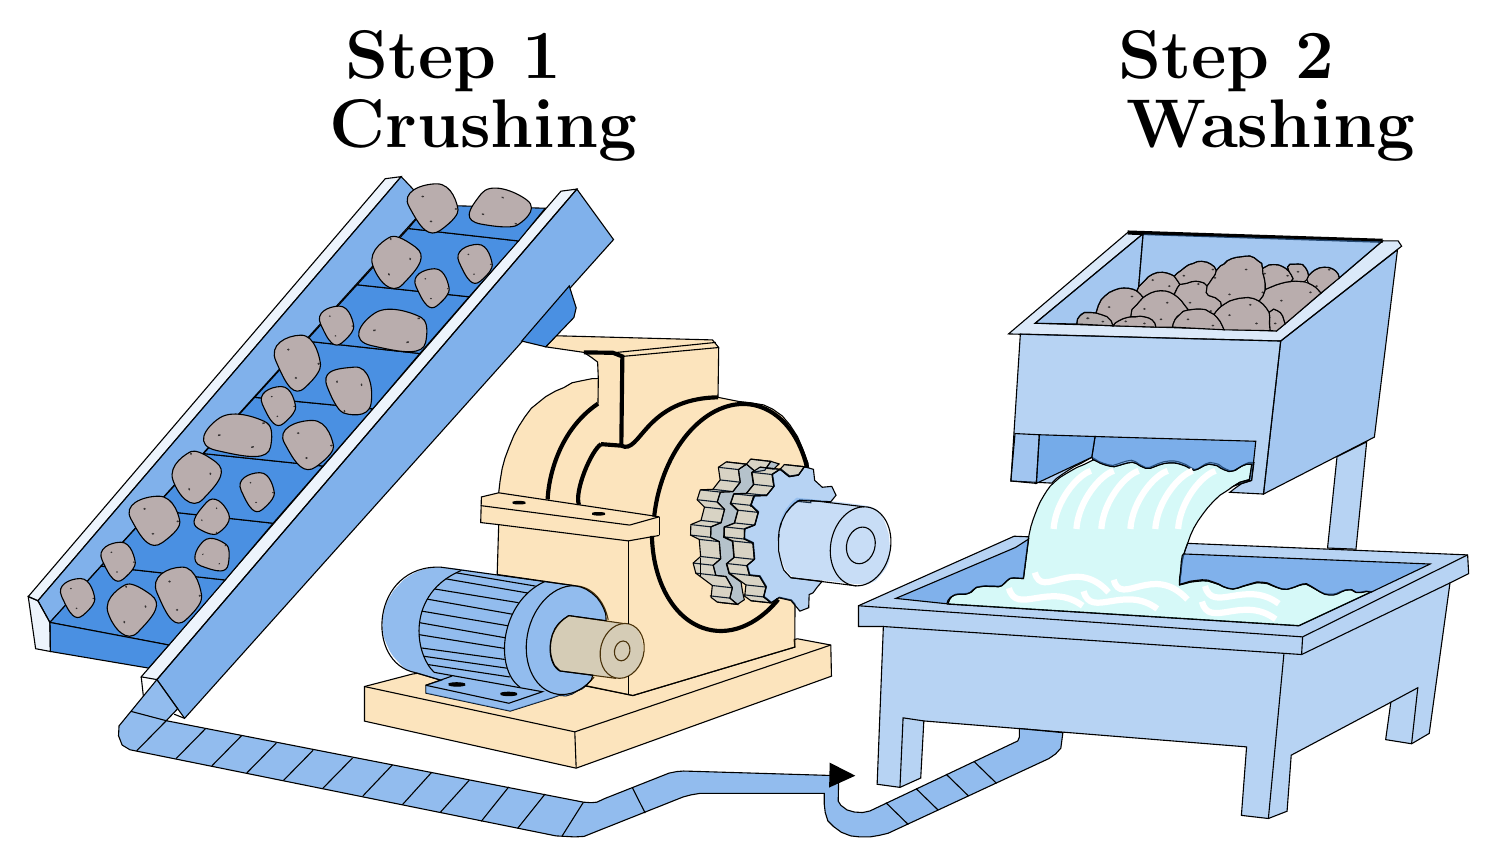
\begin{tikzpicture}[x=0.75pt,y=0.75pt,yscale=-1,xscale=1]
			%uncomment if require: \path (0,439); %set diagram left start at 0, and has height of 439
			%\draw rectangle(600,280)--(700,300) 
			%Shape: Path Data [id:dp47998155592793723] 
			\draw  [fill={rgb, 255:red, 74; green, 144; blue, 226 }  ,fill opacity=0.4 ] (436,303.25) -- (436,293.25) -- (511,259.75) -- (518.02,260.04) -- (515.43,280.04) -- (512.66,279.88) -- (510.81,279.73) -- (508.97,280.04) -- (507.58,281.12) -- (506.35,282.35) -- (505.12,283.42) -- (503.58,283.88) -- (501.58,283.73) -- (499.58,283.73) -- (497.43,283.58) -- (494.97,283.88) -- (493.12,284.19) -- (491.73,285.27) -- (490.5,286.5) -- (488.66,287.27) -- (486.97,287.42) -- (484.81,287.42) -- (482.81,287.73) -- (480.97,288.81) -- (479.89,290.19) -- (479.12,292.35) -- (648.2,302.81) -- (683.12,286.5) -- (680.5,286.19) -- (678.04,286.65) -- (675.58,286.65) -- (673.43,285.42) -- (670.66,285.58) -- (668.5,286.35) -- (666.5,287.27) -- (664.66,287.73) -- (662.66,287.73) -- (660.5,287.42) -- (658.2,286.35) -- (656.35,285.27) -- (654.2,284.04) -- (651.73,282.81) -- (649.89,282.96) -- (648.2,283.42) -- (646.2,284.19) -- (644.2,284.81) -- (642.35,285.27) -- (640.04,285.12) -- (637.58,284.35) -- (635.27,283.42) -- (633.12,282.5) -- (630.81,282.19) -- (628.04,282.04) -- (625.58,282.65) -- (623.27,283.27) -- (621.12,283.88) -- (618.81,284.65) -- (616.5,285.12) -- (614.2,284.81) -- (611.89,284.04) -- (609.73,282.96) -- (606.97,282.04) -- (604.5,281.27) -- (601.73,281.12) -- (598.81,281.42) -- (596.04,281.73) -- (593.27,282.5) -- (590.81,283.12) -- (590.97,280.19) -- (591.43,277.12) -- (591.73,273.42) -- (592.35,269.88) -- (593.43,266.35) -- (594.57,263.19) -- (729.5,268.75) -- (730,277.75) -- (721,282.25) -- (711,354.75) -- (702.5,359.75) -- (690,357.75) -- (692.5,339.75) -- (644.5,365.25) -- (642.5,392.25) -- (633.5,395.75) -- (620.5,394.25) -- (623,361.25) -- (467.5,348.75) -- (466,376.25) -- (456,380.75) -- (445,379.25) -- (448,303.25) -- (436,303.25) -- cycle ;
			%Straight Lines [id:da6371574232757211] 
			\draw    (456,380.75) -- (457.5,347.25) -- (467.5,348.75) ;
			%Straight Lines [id:da8576738355952166] 
			\draw    (702.5,359.75) -- (705.5,332.75) -- (692.5,339.75) ;
			%Straight Lines [id:da9883611962258015] 
			\draw    (448,303.25) -- (649.5,316.75) ;
			%Straight Lines [id:da6173299361875831] 
			\draw    (633.5,395.75) -- (641,316.25) ;
			%Straight Lines [id:da8227739494986746] 
			\draw    (721,282.25) -- (649.5,316.75) ;
			%Straight Lines [id:da49053920817500674] 
			\draw    (729.5,268.75) -- (650,308.25) ;
			%Straight Lines [id:da06166389805806527] 
			\draw    (650,308.25) -- (436,293.25) ;
			%Straight Lines [id:da522774026935622] 
			\draw    (649.5,316.75) -- (650,308.25) ;
			%Shape: Path Data [id:dp578935762033835] 
			\draw  [fill={rgb, 255:red, 245; green, 166; blue, 35 }  ,fill opacity=0.3 ] (198,348.83) -- (198,332.17) -- (221,326.17) -- (223.62,325.78) -- (235,329.17) -- (227.56,331.56) -- (227.56,335.33) -- (268.22,344) -- (288.67,337.56) -- (291.78,336.44) -- (295.11,336.67) -- (298,335.78) -- (300.67,334.22) -- (303.11,333.11) -- (304.67,331.71) -- (306.67,332.17) -- (327.33,336.5) -- (405.33,313.17) -- (405,309.5) -- (406.67,309.17) -- (422.67,312.17) -- (423,327.17) -- (300,371.5) -- (198,348.83) -- cycle ;
			%Shape: Polygon [id:ds8933441742073948] 
			\draw  [draw opacity=0][fill={rgb, 255:red, 74; green, 144; blue, 226 }  ,fill opacity=0.6 ] (235,329.17) -- (227.56,331.56) -- (227.56,335.33) -- (268.22,344) -- (288.67,337.56) -- (291.78,336.44) -- (295.11,336.67) -- (298,335.78) -- (300.67,334.22) -- (303.11,333.11) -- (305.33,331.11) -- (307.33,328.89) -- (308,326.67) -- (292.22,324.67) -- (289.56,322) -- (288.44,319.33) -- (287.78,316.67) -- (287.56,313.78) -- (287.78,310.67) -- (288.44,307.33) -- (289.78,304.22) -- (291.56,301.78) -- (293.78,299.78) -- (296.44,298) -- (314.44,300.44) -- (314.22,297.11) -- (313.11,294.22) -- (311.78,291.78) -- (310,289.33) -- (307.56,287.11) -- (304.89,285.33) -- (302.22,284.22) -- (299.11,283.56) -- (240.67,275.11) -- (234.89,274.67) -- (230.89,274.67) -- (226.89,275.56) -- (223.11,276.89) -- (219.78,278.67) -- (216.67,280.89) -- (214.22,283.56) -- (212,286) -- (210,289.33) -- (208.44,292.22) -- (207.56,295.56) -- (206.89,298.67) -- (206.67,302.44) -- (206.89,305.56) -- (207.33,308.44) -- (208.67,311.78) -- (210.22,315.11) -- (212,317.78) -- (214.22,320.22) -- (216.22,322.44) -- (219,324.5) -- (222.67,325.5) -- cycle ;
			%Shape: Path Data [id:dp44462219616747434] 
			\draw  [draw opacity=0][fill={rgb, 255:red, 74; green, 144; blue, 226 }  ,fill opacity=0.3 ] (314.44,300.44) -- (322.67,301.78) -- (325.78,302.44) -- (327.78,303.33) -- (329.56,304.67) -- (330.67,306.89) -- (331.56,309.56) -- (332.22,312.22) -- (332.22,317.78) -- (331.56,320.89) -- (330,323.33) -- (327.78,325.33) -- (325.33,327.33) -- (322.44,328.22) -- (319.11,328.22) -- (315.33,327.78) -- (308,326.67) -- (292.22,324.67) -- (292.22,324.67) -- (292.22,324.67) -- (289.56,322) -- (288.44,319.33) -- (287.78,316.67) -- (287.56,313.78) -- (287.78,310.67) -- (288.44,307.33) -- (289.78,304.22) -- (291.56,301.78) -- (293.78,299.78) -- (296.44,298) -- (296.44,298) -- (314.44,300.44) -- cycle ;
			%Curve Lines [id:da6717194139506665] 
			\draw    (234.89,274.67) .. controls (201.11,273.11) and (197.78,320.89) .. (222.67,325.5) ;
			%Straight Lines [id:da46273071311726655] 
			\draw    (234.89,274.67) -- (299.11,283.56) ;
			%Shape: Arc [id:dp7769717254169928] 
			\draw  [draw opacity=0] (308.64,327.59) .. controls (304.46,332.78) and (298.93,336.03) .. (293.16,336.03) .. controls (282.21,336.03) and (274.59,324.29) .. (276.14,309.81) .. controls (277.69,295.33) and (287.83,283.59) .. (298.78,283.59) .. controls (307.12,283.59) and (313.53,290.41) .. (315.43,300.07) -- (295.97,309.81) -- cycle ; \draw   (308.64,327.59) .. controls (304.46,332.78) and (298.93,336.03) .. (293.16,336.03) .. controls (282.21,336.03) and (274.59,324.29) .. (276.14,309.81) .. controls (277.69,295.33) and (287.83,283.59) .. (298.78,283.59) .. controls (307.12,283.59) and (313.53,290.41) .. (315.43,300.07) ;  
			%Straight Lines [id:da5875726230247784] 
			\draw    (231.56,325.33) -- (283.78,334.67) -- (267.56,340.22) -- (227.56,331.56) ;
			%Straight Lines [id:da7837838229514839] 
			\draw    (227.56,331.56) -- (240.22,327.11) ;
			%Shape: Circle [id:dp7289861743084469] 
			\draw  [fill={rgb, 255:red, 0; green, 0; blue, 0 }  ,fill opacity=1 ] (265.87,334.98) .. controls (267.91,334.81) and (270.3,335.01) .. (271.21,335.43) .. controls (272.12,335.84) and (271.21,336.32) .. (269.17,336.49) .. controls (267.13,336.66) and (264.74,336.46) .. (263.83,336.04) .. controls (262.91,335.63) and (263.83,335.15) .. (265.87,334.98) -- cycle ;
			%Straight Lines [id:da8972147565612089] 
			\draw    (242.22,277.38) -- (280.44,283.78) ;
			%Straight Lines [id:da5462562914455673] 
			\draw    (237.11,280.27) -- (276.67,287.11) ;
			%Straight Lines [id:da2802126647945481] 
			\draw    (231.78,285.16) -- (272.22,291.78) ;
			%Straight Lines [id:da7489400831496161] 
			\draw    (228.22,290.05) -- (269.33,297.33) ;
			%Straight Lines [id:da9886561024879796] 
			\draw    (225.56,295.82) -- (267.11,302.89) ;
			%Straight Lines [id:da12440342435271423] 
			\draw    (224.44,301.38) -- (265.78,308.67) ;
			%Straight Lines [id:da113949161370268] 
			\draw    (224.22,307.16) -- (265.33,313.78) ;
			%Straight Lines [id:da9422162798634979] 
			\draw    (225.56,313.6) -- (265.56,319.11) ;
			%Straight Lines [id:da7480814468384397] 
			\draw    (226.67,317.6) -- (266.67,323.33) ;
			%Straight Lines [id:da8680337856567306] 
			\draw    (228.67,321.6) -- (268,327.56) ;
			%Curve Lines [id:da0759229297335352] 
			\draw    (296.44,298) .. controls (283.78,305.56) and (286.44,322.22) .. (292.22,324.67) ;
			%Curve Lines [id:da38902220359502393] 
			\draw    (284.89,281.56) .. controls (263.11,291.56) and (260.44,323.56) .. (272.89,332.44) ;
			%Curve Lines [id:da6712637701486416] 
			\draw    (244.67,276.22) .. controls (218.22,287.33) and (221.78,316) .. (231.56,325.33) ;
			%Straight Lines [id:da13614991463095105] 
			\draw    (296.44,298) -- (322.67,301.78) ;
			%Straight Lines [id:da6845540821851183] 
			\draw    (292.22,324.67) -- (319.11,328.22) ;
			%Shape: Ellipse [id:dp6934622203621525] 
			\draw   (311.61,315) .. controls (312.32,307.7) and (317.62,301.78) .. (323.45,301.78) .. controls (329.28,301.78) and (333.43,307.7) .. (332.72,315) .. controls (332.01,322.3) and (326.71,328.22) .. (320.88,328.22) .. controls (315.05,328.22) and (310.9,322.3) .. (311.61,315) -- cycle ;
			%Straight Lines [id:da46413413302800965] 
			\draw    (222.67,325.5) -- (235,329.17) ;
			%Straight Lines [id:da27277691982925334] 
			\draw    (198,332.17) -- (299.33,354) ;
			%Straight Lines [id:da735702473973795] 
			\draw    (300,371.5) -- (299.33,354) ;
			%Straight Lines [id:da6133596088156593] 
			\draw    (299.33,354) -- (422.67,312.17) ;
			%Shape: Ellipse [id:dp651804606290438] 
			\draw   (318.44,315) .. controls (318.7,312.36) and (320.57,310.22) .. (322.63,310.22) .. controls (324.68,310.22) and (326.14,312.36) .. (325.89,315) .. controls (325.63,317.64) and (323.76,319.78) .. (321.7,319.78) .. controls (319.65,319.78) and (318.19,317.64) .. (318.44,315) -- cycle ;
			%Shape: Path Data [id:dp3373436424703994] 
			\draw  [fill={rgb, 255:red, 245; green, 166; blue, 35 }  ,fill opacity=0.3 ] (405.33,313.17) -- (327.33,336.5) -- (304.46,331.9) -- (305.33,331.11) -- (307.33,328.89) -- (308,326.67) -- (292.22,324.67) -- (289.56,322) -- (288.44,319.33) -- (287.78,316.67) -- (287.56,313.78) -- (287.78,310.67) -- (288.44,307.33) -- (289.78,304.22) -- (291.56,301.78) -- (293.78,299.78) -- (296.44,298) -- (314.44,300.44) -- (314.22,297.11) -- (313.11,294.22) -- (311.78,291.78) -- (310,289.33) -- (307.56,287.11) -- (304.89,285.33) -- (302.22,284.22) -- (299.11,283.56) -- (261.96,278.19) -- (262,276.17) -- (262.67,254.17) -- (254,253.17) -- (254.33,240.83) -- (262.67,238.83) -- (263.33,233.17) -- (264.33,227.17) -- (265.67,222.17) -- (267.67,216.83) -- (270,211.17) -- (272.33,206.83) -- (275.33,202.17) -- (278.33,198.17) -- (282,195.17) -- (285.33,192.5) -- (290,189.83) -- (294,188.17) -- (298,185.83) -- (302.67,184.83) -- (307.67,183.83) -- (310.67,183.83) -- (310.33,175.83) -- (307.67,173.83) -- (303.67,171.17) -- (285.33,168.5) -- (290.33,163.17) -- (365.67,165.17) -- (368.67,168.83) -- (368.33,192.83) -- (378.33,194.83) -- (384.33,195.5) -- (390.33,196.5) -- (394.67,198.5) -- (399.33,201.83) -- (403,206.17) -- (406.67,211.83) -- (409.33,218.17) -- (411.67,224.5) -- (411.9,226.48) -- (410.18,225.98) -- (407.28,230.05) -- (402.86,230.78) -- (398.46,227.24) -- (394.59,229.73) -- (395.46,235.53) -- (391.95,239.83) -- (385.9,240.08) -- (384.37,244.61) -- (387.9,247.98) -- (386.23,254.1) -- (381.34,256.01) -- (381.19,260.82) -- (385.37,262.8) -- (386.05,270.64) -- (382.45,273.66) -- (383.7,278.29) -- (388.57,278.82) -- (391.67,283.98) -- (390.5,288.72) -- (394.11,291.6) -- (397.9,289.15) -- (403.71,290.47) -- (405.43,292.5) -- (405.33,313.17) -- cycle (413,243.6) -- (406.41,242.93) -- (403.43,245.66) -- (401.24,248.39) -- (401.24,248.39) -- (403.06,246.03) -- (403.43,245.66) -- (403.66,245.38) -- (404.33,244.76) -- (405.42,243.67) -- (405.72,243.49) -- (406.63,242.65) -- (407.02,242.69) -- (407.7,242.27) -- (413,242.46) -- (413,243.6) -- cycle (397.67,260.17) -- (397.82,258.61) -- (397.68,260.37) -- (397.67,260.17) -- cycle (398.7,253.85) -- (398.9,253.37) -- (398.33,255.49) -- (398.7,253.85) -- cycle ;
			%Shape: Polygon [id:ds388190504952024] 
			\draw  [fill={rgb, 255:red, 50; green, 226; blue, 220 }  ,fill opacity=0.2 ] (625.71,224.93) -- (624.57,232.36) -- (619.85,233.69) -- (616.62,235.69) -- (613.54,237.85) -- (610.15,240) -- (606.92,243.08) -- (604.15,246.15) -- (601.69,249.38) -- (599.54,252.46) -- (597.54,255.85) -- (596,259.23) -- (594.62,263.08) -- (593.38,266.46) -- (592.31,270) -- (591.69,273.54) -- (591.38,277.23) -- (590.92,280.31) -- (590.77,283.23) -- (593.23,282.62) -- (596,281.85) -- (598.77,281.54) -- (601.69,281.23) -- (604.46,281.38) -- (606.92,282.15) -- (609.69,283.08) -- (611.85,284.15) -- (614.15,284.92) -- (616.46,285.23) -- (618.77,284.77) -- (621.08,284) -- (623.23,283.38) -- (625.54,282.77) -- (628,282.15) -- (630.77,282.31) -- (633.08,282.62) -- (635.23,283.54) -- (637.54,284.46) -- (640,285.23) -- (642.31,285.38) -- (644.15,284.92) -- (646.15,284.31) -- (648.15,283.54) -- (649.85,283.08) -- (651.69,282.92) -- (654.15,284.15) -- (656.31,285.38) -- (658.15,286.46) -- (660.46,287.54) -- (662.62,287.85) -- (664.62,287.85) -- (666.46,287.38) -- (668.46,286.46) -- (670.62,285.69) -- (673.38,285.54) -- (675.54,286.77) -- (678,286.77) -- (680.46,286.31) -- (683.08,286.62) -- (648.15,302.92) -- (479.08,292.46) -- (479.85,290.31) -- (480.92,288.92) -- (482.77,287.85) -- (484.77,287.54) -- (486.92,287.54) -- (488.62,287.38) -- (490.46,286.62) -- (491.69,285.38) -- (493.08,284.31) -- (494.92,284) -- (497.38,283.69) -- (499.54,283.85) -- (501.54,283.85) -- (503.54,284) -- (505.08,283.54) -- (506.31,282.46) -- (507.54,281.23) -- (508.92,280.15) -- (510.77,279.85) -- (512.62,280) -- (515.38,280.15) -- (518,260) -- (519.08,255.08) -- (520.15,251.69) -- (521.23,248.77) -- (522.31,246) -- (523.54,243.23) -- (525.23,240.31) -- (526.77,237.85) -- (528.46,235.54) -- (530.62,233.54) -- (532.92,231.54) -- (535.38,230) -- (538,228.46) -- (541.23,226.62) -- (544.62,225.23) -- (547.08,224) -- (549.54,222.77) -- (551.08,223.54) -- (552.77,224.46) -- (554.92,225.23) -- (557.23,225.85) -- (559.38,226.15) -- (561.69,225.54) -- (563.69,224.92) -- (566,224.31) -- (568.15,224) -- (570.15,224.62) -- (572.15,225.85) -- (574.62,226.92) -- (576.77,226.92) -- (578.77,226.15) -- (580.77,225.38) -- (583.38,224.62) -- (585.85,224.31) -- (588.31,224.31) -- (590.15,224.62) -- (592.15,225.23) -- (593.85,225.85) -- (595.85,226.92) -- (597.85,227.85) -- (599.54,227.38) -- (601.23,226.46) -- (602.92,225.54) -- (605.08,224.92) -- (607.08,225.23) -- (609.08,225.69) -- (610.92,226.92) -- (612.62,227.69) -- (614.77,228.46) -- (617.14,228.07) -- (619,226.93) -- (621,225.79) -- (623.29,224.93) -- cycle ;
			%Shape: Path Data [id:dp37098655363060096] 
			\draw  [fill={rgb, 255:red, 74; green, 144; blue, 226 }  ,fill opacity=0.5 ] (454,289.71) -- (511.71,265.14) -- (517.99,261.11) -- (515.54,280.15) -- (512.71,279.99) -- (510.81,279.84) -- (508.92,280.15) -- (507.5,281.27) -- (506.24,282.54) -- (504.98,283.66) -- (503.41,284.14) -- (501.36,283.98) -- (499.31,283.98) -- (497.1,283.82) -- (494.58,284.14) -- (492.69,284.46) -- (491.27,285.57) -- (490.01,286.84) -- (488.12,287.64) -- (486.39,287.8) -- (484.18,287.8) -- (482.13,288.12) -- (480.24,289.23) -- (479.14,290.67) -- (478.57,292.29) -- (454,289.71) -- cycle ;
			%Shape: Path Data [id:dp2265293061389051] 
			\draw  [fill={rgb, 255:red, 74; green, 144; blue, 226 }  ,fill opacity=0.5 ] (592.57,268.29) -- (711.43,273.14) -- (683.02,286.68) -- (680.8,286.39) -- (678.32,286.91) -- (675.85,286.91) -- (673.68,285.53) -- (670.89,285.7) -- (668.73,286.56) -- (666.72,287.59) -- (664.86,288.11) -- (662.85,288.11) -- (660.68,287.76) -- (658.36,286.56) -- (656.5,285.36) -- (654.34,283.99) -- (651.86,282.61) -- (650,282.78) -- (648.3,283.3) -- (646.29,284.16) -- (644.28,284.85) -- (642.42,285.36) -- (640.1,285.19) -- (637.63,284.33) -- (635.3,283.3) -- (633.14,282.27) -- (630.82,281.93) -- (628.03,281.75) -- (625.56,282.44) -- (623.24,283.13) -- (621.07,283.82) -- (618.75,284.67) -- (616.43,285.19) -- (614.11,284.85) -- (611.78,283.99) -- (609.62,282.78) -- (606.83,281.75) -- (604.36,280.9) -- (601.57,280.72) -- (598.63,281.07) -- (595.85,281.41) -- (593.06,282.27) -- (590.59,282.96) -- (590.74,279.69) -- (591.2,276.26) -- (591.51,272.14) -- (591.99,269.11) -- (592.57,268.29) -- cycle ;
			%Shape: Polygon [id:ds49575820102032786] 
			\draw  [fill={rgb, 255:red, 74; green, 144; blue, 226 }  ,fill opacity=0.4 ] (680.86,214.29) -- (675.71,266) -- (662,265.43) -- (666.57,221.43) -- cycle ;
			%Shape: Polygon [id:ds15794886002080666] 
			\draw  [fill={rgb, 255:red, 74; green, 144; blue, 226 }  ,fill opacity=0.5 ] (695.71,121.71) -- (684.57,212) -- (631.14,239.43) -- (639.43,165.71) -- cycle ;
			%Shape: Polygon [id:ds48069844422252694] 
			\draw  [fill={rgb, 255:red, 74; green, 144; blue, 226 }  ,fill opacity=0.2 ] (697.71,120) -- (696,117.43) -- (688.57,117.43) -- (637.43,160.86) -- (521.14,157.14) -- (573.14,114) -- (565.71,113.43) -- (508.29,162.29) -- (639.43,165.71) -- cycle ;
			%Straight Lines [id:da31547597663303173] 
			\draw [line width=1.5]    (565.71,113.43) -- (688.57,117.43) ;
			%Shape: Path Data [id:dp40821352651150644] 
			\draw  [fill={rgb, 255:red, 74; green, 144; blue, 226 }  ,fill opacity=0.4 ] (631.14,239.43) -- (614.94,238.59) -- (617.24,236.77) -- (620.55,234.44) -- (625.4,232.88) -- (626.57,224.23) -- (624.08,224.23) -- (621.74,225.23) -- (619.68,226.56) -- (617.78,227.89) -- (615.34,228.34) -- (613.13,227.45) -- (611.4,226.55) -- (609.5,225.12) -- (607.45,224.58) -- (605.4,224.22) -- (603.19,224.94) -- (599.72,227.09) -- (597.98,227.63) -- (595.93,226.55) -- (593.88,225.3) -- (592.14,224.58) -- (590.09,223.86) -- (588.2,223.51) -- (585.67,223.51) -- (583.15,223.86) -- (580.47,224.76) -- (576.36,226.55) -- (574.15,226.55) -- (571.63,225.3) -- (569.58,223.86) -- (567.52,223.15) -- (565.32,223.51) -- (562.95,224.22) -- (560.9,224.94) -- (558.53,225.66) -- (556.32,225.3) -- (553.95,224.58) -- (551.74,223.69) -- (550.01,222.61) -- (548.43,221.71) -- (543.38,224.58) -- (539.91,226.19) -- (536.59,228.34) -- (533.91,230.14) -- (531.38,231.93) -- (529.12,234.16) -- (509.43,233.14) -- (514,162.34) -- (639.43,165.71) -- (631.14,239.43) -- cycle ;
			%Shape: Path Data [id:dp130801383546857] 
			\draw  [fill={rgb, 255:red, 74; green, 144; blue, 226 }  ,fill opacity=0.55 ] (625.4,232.88) -- (616.88,235.53) -- (619.59,233.85) -- (624.31,232.52) -- (625.45,225.09) -- (623.03,225.09) -- (620.74,225.95) -- (618.74,227.09) -- (616.88,228.23) -- (614.51,228.62) -- (612.36,227.85) -- (610.66,227.08) -- (608.82,225.85) -- (606.82,225.39) -- (604.82,225.08) -- (602.66,225.7) -- (599.28,227.55) -- (597.59,228.01) -- (595.59,227.08) -- (593.59,226.01) -- (591.89,225.39) -- (589.89,224.78) -- (588.05,224.47) -- (585.59,224.47) -- (583.12,224.78) -- (580.51,225.55) -- (576.51,227.08) -- (574.36,227.08) -- (571.89,226.01) -- (569.89,224.78) -- (567.89,224.16) -- (565.74,224.47) -- (563.43,225.08) -- (561.43,225.7) -- (559.12,226.31) -- (556.97,226.01) -- (554.66,225.39) -- (552.51,224.62) -- (550.82,223.7) -- (549.28,222.93) -- (548.98,223.08) -- (548.43,221.71) -- (550,211.71) -- (627.43,214) -- (625.4,232.88) -- cycle ;
			%Shape: Polygon [id:ds9353418031708952] 
			\draw  [fill={rgb, 255:red, 74; green, 144; blue, 226 }  ,fill opacity=0.6 ] (550,211.71) -- (548.43,221.71) -- (521.71,234.29) -- (523.14,210.86) -- cycle ;
			%Shape: Polygon [id:ds04923347788783161] 
			\draw  [fill={rgb, 255:red, 74; green, 144; blue, 226 }  ,fill opacity=0.2 ] (523.14,210.86) -- (521.71,234.29) -- (509.43,233.14) -- (511.43,210.29) -- cycle ;
			%Shape: Polygon [id:ds11080967295601374] 
			\draw  [fill={rgb, 255:red, 180; green, 173; blue, 173 }  ,fill opacity=1 ] (543.11,152.83) -- (544.89,151.94) -- (547.78,151.94) -- (550.44,152.17) -- (553.33,153.06) -- (555.78,153.94) -- (557.78,155.94) -- (558.67,158.39) -- (541.16,157.5) -- (541.56,155.06) -- cycle ;
			%Shape: Polygon [id:ds6565093448724328] 
			\draw  [fill={rgb, 255:red, 185; green, 173; blue, 173 }  ,fill opacity=1 ] (561.29,156) -- (563.29,155) -- (565.14,154.43) -- (567.14,154) -- (569.57,154) -- (571.71,153.71) -- (573.71,154) -- (575.86,154.57) -- (577.57,155.57) -- (578.86,157.14) -- (579.29,159) -- (558.67,158.39) -- (559.71,157) -- cycle ;
			%Shape: Polygon [id:ds8886409295245203] 
			\draw  [fill={rgb, 255:red, 185; green, 173; blue, 173 }  ,fill opacity=1 ] (577.57,155.57) -- (575.86,154.57) -- (573.71,154) -- (571.71,153.71) -- (569.57,154) -- (567.14,154) -- (567.71,150.57) -- (570,148.29) -- (571.43,146.57) -- (573.14,144.71) -- (574.86,143.57) -- (577,142.43) -- (579.29,141.71) -- (581.57,141.43) -- (583.86,141.57) -- (586,142.14) -- (588.14,143.29) -- (590,144.71) -- (591.71,146.43) -- (592.86,148) -- (595,150.71) -- (592.43,151.43) -- (591,152.86) -- (589.57,153.86) -- (588.57,155.29) -- (587.71,157.29) -- (587.29,159) -- (579.29,159) -- (578.86,157.14) -- cycle ;
			%Shape: Polygon [id:ds7354170031490268] 
			\draw  [fill={rgb, 255:red, 185; green, 173; blue, 173 }  ,fill opacity=1 ] (557.78,155.94) -- (555.78,153.94) -- (553.33,153.06) -- (550.44,152.17) -- (551.57,148.57) -- (553,145.71) -- (554.71,144) -- (556.86,142.29) -- (559,141.29) -- (561.43,140.43) -- (563.86,140.14) -- (566.14,140.29) -- (568.14,140.71) -- (570.14,141.57) -- (571.86,143.14) -- (573.14,144.71) -- (571.43,146.57) -- (570,148.29) -- (567.71,150.57) -- (567.14,154) -- (565.14,154.43) -- (563.29,155) -- (561.29,156) -- (559.71,157) -- (558.67,158.39) -- cycle ;
			%Shape: Polygon [id:ds5409654681462979] 
			\draw  [fill={rgb, 255:red, 185; green, 173; blue, 173 }  ,fill opacity=1 ] (588.57,155.29) -- (590.29,153.43) -- (592.43,151.43) -- (595,150.71) -- (598.57,150.29) -- (601,150.29) -- (603.29,150.57) -- (605.43,151.86) -- (607.29,152.86) -- (608.71,154.29) -- (610.29,156.29) -- (611.29,158.29) -- (612.14,160.29) -- (587.29,159) -- (587.71,157.29) -- cycle ;
			%Shape: Polygon [id:ds6956573743010264] 
			\draw  [fill={rgb, 255:red, 185; green, 173; blue, 173 }  ,fill opacity=1 ] (570.14,141.57) -- (571,139.57) -- (573.57,137) -- (575.71,134.71) -- (577.86,133.43) -- (580,132.71) -- (582.43,132.57) -- (584.43,132.86) -- (586.43,133.57) -- (588.14,134.43) -- (589.86,136.86) -- (590.86,138.43) -- (589.71,140) -- (588.86,141.57) -- (588.14,143.29) -- (586,142.14) -- (583.86,141.57) -- (581.57,141.43) -- (579.29,141.71) -- (577,142.43) -- (574.86,143.57) -- (573.14,144.71) -- (571.86,143.14) -- cycle ;
			%Shape: Polygon [id:ds9734189288396476] 
			\draw  [fill={rgb, 255:red, 185; green, 173; blue, 173 }  ,fill opacity=1 ] (634,156.86) -- (634.14,154.29) -- (633.86,151.86) -- (636,150.29) -- (637.71,151) -- (639.29,152) -- (640.43,153.71) -- (641,155.57) -- (641.57,157.43) -- (637.43,160.86) -- (634.29,160.71) -- (634.14,158.86) -- cycle ;
			%Shape: Polygon [id:ds5541066229842778] 
			\draw  [fill={rgb, 255:red, 185; green, 173; blue, 173 }  ,fill opacity=1 ] (610.29,156.29) -- (608.71,154.29) -- (607.29,152.86) -- (608.29,151.43) -- (609.57,150) -- (610.86,148.86) -- (612.86,147.57) -- (614.71,146.43) -- (617,145.71) -- (619.29,145.14) -- (621.71,144.86) -- (623.86,144.71) -- (626.57,145.29) -- (629,146.43) -- (631,148) -- (632.57,149.86) -- (633.86,151.86) -- (634.14,154.29) -- (634,156.86) -- (634.14,158.86) -- (634.29,160.71) -- (612.14,160.29) -- (611.29,158.29) -- cycle ;
			%Shape: Polygon [id:ds42060158468465747] 
			\draw  [fill={rgb, 255:red, 185; green, 173; blue, 173 }  ,fill opacity=1 ] (632,140.86) -- (634,140) -- (637.14,138.71) -- (639.86,137.86) -- (642.29,137.29) -- (644.43,137) -- (646.43,136.86) -- (648.71,137) -- (650.86,137.14) -- (652.86,137.86) -- (654.57,138.71) -- (656.14,139.71) -- (657.57,141.14) -- (658.86,142.57) -- (641.57,157.43) -- (641,155.57) -- (640.43,153.71) -- (639.29,152) -- (637.71,151) -- (636,150.29) -- (633.86,151.86) -- (632.57,149.86) -- (631,148) -- (629,146.43) -- (630.86,144) -- cycle ;
			%Shape: Polygon [id:ds4996369651003628] 
			\draw  [fill={rgb, 255:red, 185; green, 173; blue, 173 }  ,fill opacity=1 ] (591.71,146.43) -- (590,144.71) -- (588.14,143.29) -- (589.71,140) -- (590.86,138.43) -- (594.29,137.86) -- (596.43,137.14) -- (598.57,136.86) -- (600.57,137.14) -- (602.43,137.71) -- (604,139.14) -- (603.86,140.57) -- (603.57,142.29) -- (604.57,143.71) -- (606.29,144.29) -- (608,144.86) -- (609.43,146) -- (610.57,147) -- (610.86,148.86) -- (609.57,150) -- (608.29,151.43) -- (607.29,152.86) -- (605.43,151.86) -- (603.29,150.57) -- (601,150.29) -- (598.57,150.29) -- (595,150.71) -- (592.86,148) -- cycle ;
			%Shape: Polygon [id:ds9387668418366766] 
			\draw  [fill={rgb, 255:red, 185; green, 173; blue, 173 }  ,fill opacity=1 ] (588.14,134.43) -- (589.57,133) -- (591.43,131.71) -- (593.14,130.29) -- (595,129) -- (597.29,128.29) -- (599.29,127.43) -- (601.43,127.29) -- (603.86,127.71) -- (605.86,128.71) -- (607.43,129.86) -- (608.43,131.71) -- (607.86,133.71) -- (606.43,135.71) -- (605.29,137.43) -- (604,139.14) -- (602.43,137.71) -- (600.57,137.14) -- (598.57,136.86) -- (596.43,137.14) -- (594.29,137.86) -- (590.86,138.43) -- (589.86,136.86) -- cycle ;
			%Shape: Polygon [id:ds3545544912602966] 
			\draw  [fill={rgb, 255:red, 185; green, 173; blue, 173 }  ,fill opacity=1 ] (609.43,146) -- (608,144.86) -- (606.29,144.29) -- (604.57,143.71) -- (603.57,142.29) -- (604,139.14) -- (605.29,137.43) -- (606.43,135.71) -- (607.86,133.71) -- (608.43,131.71) -- (610.29,129.57) -- (612.14,128.57) -- (613.71,127) -- (615.86,126) -- (617.86,125.43) -- (620.14,125.14) -- (622.29,124.86) -- (624.57,124.71) -- (626.71,125.57) -- (628.43,127) -- (630.29,128.29) -- (630.71,130.71) -- (630.86,133) -- (631.57,135.57) -- (632,138.14) -- (632,140.86) -- (630.86,144) -- (629,146.43) -- (626.57,145.29) -- (623.86,144.71) -- (621.71,144.86) -- (619.29,145.14) -- (617,145.71) -- (614.71,146.43) -- (612.86,147.57) -- (610.86,148.86) -- (610.57,147) -- cycle ;
			%Shape: Polygon [id:ds5363086427524476] 
			\draw  [fill={rgb, 255:red, 185; green, 173; blue, 173 }  ,fill opacity=1 ] (631.57,135.57) -- (630.86,133) -- (630.71,130.71) -- (633.86,129) -- (636.14,128.86) -- (638.29,129) -- (640.14,129.71) -- (641.86,130.71) -- (643.29,132) -- (644.57,133.86) -- (645.43,135.71) -- (644.43,137) -- (642.29,137.29) -- (639.86,137.86) -- (637.14,138.71) -- (634,140) -- (632,140.86) -- (632,138.14) -- cycle ;
			%Shape: Polygon [id:ds22275363056071973] 
			\draw  [fill={rgb, 255:red, 185; green, 173; blue, 173 }  ,fill opacity=1 ] (660.43,130.14) -- (662.71,130.29) -- (664.57,131) -- (666,132) -- (667.14,133.43) -- (667.71,135.29) -- (658.86,142.57) -- (657.57,141.14) -- (656.14,139.71) -- (654.57,138.71) -- (652.86,137.86) -- (652,136.14) -- (652.86,134.14) -- (654.43,132.57) -- (656,131.43) -- (658.14,130.43) -- cycle ;
			%Shape: Polygon [id:ds04341508574356412] 
			\draw  [fill={rgb, 255:red, 185; green, 173; blue, 173 }  ,fill opacity=1 ] (644.57,133.86) -- (643.29,132) -- (642.71,130) -- (643.86,128.71) -- (645.86,128.71) -- (647.86,128.57) -- (650,128.86) -- (651.43,130.43) -- (652.43,132.29) -- (652.86,134.14) -- (652,136.14) -- (650.86,137.14) -- (648.71,137) -- (646.43,136.86) -- (644.43,137) -- (645.43,135.71) -- cycle ;
			%Shape: Ellipse [id:dp3914450157053826] 
			\draw  [draw opacity=0][fill={rgb, 255:red, 0; green, 0; blue, 0 }  ,fill opacity=0.7 ] (545.64,154.73) .. controls (545.64,154.45) and (546.02,154.23) .. (546.5,154.23) .. controls (546.98,154.23) and (547.36,154.45) .. (547.36,154.73) .. controls (547.36,155) and (546.98,155.23) .. (546.5,155.23) .. controls (546.02,155.23) and (545.64,155) .. (545.64,154.73) -- cycle ;
			%Shape: Ellipse [id:dp8401736115581442] 
			\draw  [draw opacity=0][fill={rgb, 255:red, 0; green, 0; blue, 0 }  ,fill opacity=0.7 ] (553.09,156.34) .. controls (553.09,156.08) and (553.4,155.86) .. (553.77,155.86) .. controls (554.15,155.86) and (554.45,156.08) .. (554.45,156.34) .. controls (554.45,156.6) and (554.15,156.81) .. (553.77,156.81) .. controls (553.4,156.81) and (553.09,156.6) .. (553.09,156.34) -- cycle ;
			%Shape: Ellipse [id:dp6657626785974294] 
			\draw  [draw opacity=0][fill={rgb, 255:red, 0; green, 0; blue, 0 }  ,fill opacity=0.7 ] (573.09,157.25) .. controls (573.09,156.98) and (573.4,156.77) .. (573.77,156.77) .. controls (574.15,156.77) and (574.45,156.98) .. (574.45,157.25) .. controls (574.45,157.51) and (574.15,157.72) .. (573.77,157.72) .. controls (573.4,157.72) and (573.09,157.51) .. (573.09,157.25) -- cycle ;
			%Shape: Ellipse [id:dp21320101848846096] 
			\draw  [draw opacity=0][fill={rgb, 255:red, 0; green, 0; blue, 0 }  ,fill opacity=0.7 ] (564.09,156.25) .. controls (564.09,155.98) and (564.4,155.77) .. (564.77,155.77) .. controls (565.15,155.77) and (565.45,155.98) .. (565.45,156.25) .. controls (565.45,156.51) and (565.15,156.72) .. (564.77,156.72) .. controls (564.4,156.72) and (564.09,156.51) .. (564.09,156.25) -- cycle ;
			%Shape: Ellipse [id:dp6344186090871343] 
			\draw  [draw opacity=0][fill={rgb, 255:red, 0; green, 0; blue, 0 }  ,fill opacity=0.7 ] (573.09,150.25) .. controls (573.09,149.98) and (573.4,149.77) .. (573.77,149.77) .. controls (574.15,149.77) and (574.45,149.98) .. (574.45,150.25) .. controls (574.45,150.51) and (574.15,150.72) .. (573.77,150.72) .. controls (573.4,150.72) and (573.09,150.51) .. (573.09,150.25) -- cycle ;
			%Shape: Ellipse [id:dp699682087833608] 
			\draw  [draw opacity=0][fill={rgb, 255:red, 0; green, 0; blue, 0 }  ,fill opacity=0.7 ] (581.09,155.25) .. controls (581.09,154.98) and (581.4,154.77) .. (581.77,154.77) .. controls (582.15,154.77) and (582.45,154.98) .. (582.45,155.25) .. controls (582.45,155.51) and (582.15,155.72) .. (581.77,155.72) .. controls (581.4,155.72) and (581.09,155.51) .. (581.09,155.25) -- cycle ;
			%Shape: Ellipse [id:dp7735611230182997] 
			\draw  [draw opacity=0][fill={rgb, 255:red, 0; green, 0; blue, 0 }  ,fill opacity=0.7 ] (584.09,147.25) .. controls (584.09,146.98) and (584.4,146.77) .. (584.77,146.77) .. controls (585.15,146.77) and (585.45,146.98) .. (585.45,147.25) .. controls (585.45,147.51) and (585.15,147.72) .. (584.77,147.72) .. controls (584.4,147.72) and (584.09,147.51) .. (584.09,147.25) -- cycle ;
			%Shape: Ellipse [id:dp7480055911845965] 
			\draw  [draw opacity=0][fill={rgb, 255:red, 0; green, 0; blue, 0 }  ,fill opacity=0.7 ] (556.09,149.34) .. controls (556.09,149.08) and (556.4,148.86) .. (556.77,148.86) .. controls (557.15,148.86) and (557.45,149.08) .. (557.45,149.34) .. controls (557.45,149.6) and (557.15,149.81) .. (556.77,149.81) .. controls (556.4,149.81) and (556.09,149.6) .. (556.09,149.34) -- cycle ;
			%Shape: Ellipse [id:dp629955609465148] 
			\draw  [draw opacity=0][fill={rgb, 255:red, 0; green, 0; blue, 0 }  ,fill opacity=0.7 ] (567.09,144.25) .. controls (567.09,143.98) and (567.4,143.77) .. (567.77,143.77) .. controls (568.15,143.77) and (568.45,143.98) .. (568.45,144.25) .. controls (568.45,144.51) and (568.15,144.72) .. (567.77,144.72) .. controls (567.4,144.72) and (567.09,144.51) .. (567.09,144.25) -- cycle ;
			%Shape: Ellipse [id:dp6881728885524818] 
			\draw  [draw opacity=0][fill={rgb, 255:red, 0; green, 0; blue, 0 }  ,fill opacity=0.7 ] (594.09,155.25) .. controls (594.09,154.98) and (594.4,154.77) .. (594.77,154.77) .. controls (595.15,154.77) and (595.45,154.98) .. (595.45,155.25) .. controls (595.45,155.51) and (595.15,155.72) .. (594.77,155.72) .. controls (594.4,155.72) and (594.09,155.51) .. (594.09,155.25) -- cycle ;
			%Shape: Ellipse [id:dp08232102110788442] 
			\draw  [draw opacity=0][fill={rgb, 255:red, 0; green, 0; blue, 0 }  ,fill opacity=0.7 ] (606.09,158.25) .. controls (606.09,157.98) and (606.4,157.77) .. (606.77,157.77) .. controls (607.15,157.77) and (607.45,157.98) .. (607.45,158.25) .. controls (607.45,158.51) and (607.15,158.72) .. (606.77,158.72) .. controls (606.4,158.72) and (606.09,158.51) .. (606.09,158.25) -- cycle ;
			%Shape: Ellipse [id:dp31092818471742767] 
			\draw  [draw opacity=0][fill={rgb, 255:red, 0; green, 0; blue, 0 }  ,fill opacity=0.7 ] (614.09,153.25) .. controls (614.09,152.98) and (614.4,152.77) .. (614.77,152.77) .. controls (615.15,152.77) and (615.45,152.98) .. (615.45,153.25) .. controls (615.45,153.51) and (615.15,153.72) .. (614.77,153.72) .. controls (614.4,153.72) and (614.09,153.51) .. (614.09,153.25) -- cycle ;
			%Shape: Ellipse [id:dp8954603368031052] 
			\draw  [draw opacity=0][fill={rgb, 255:red, 0; green, 0; blue, 0 }  ,fill opacity=0.7 ] (627.09,157.25) .. controls (627.09,156.98) and (627.4,156.77) .. (627.77,156.77) .. controls (628.15,156.77) and (628.45,156.98) .. (628.45,157.25) .. controls (628.45,157.51) and (628.15,157.72) .. (627.77,157.72) .. controls (627.4,157.72) and (627.09,157.51) .. (627.09,157.25) -- cycle ;
			%Shape: Ellipse [id:dp8669873435716808] 
			\draw  [draw opacity=0][fill={rgb, 255:red, 0; green, 0; blue, 0 }  ,fill opacity=0.7 ] (624.09,148.25) .. controls (624.09,147.98) and (624.4,147.77) .. (624.77,147.77) .. controls (625.15,147.77) and (625.45,147.98) .. (625.45,148.25) .. controls (625.45,148.51) and (625.15,148.72) .. (624.77,148.72) .. controls (624.4,148.72) and (624.09,148.51) .. (624.09,148.25) -- cycle ;
			%Shape: Ellipse [id:dp5112268216132019] 
			\draw  [draw opacity=0][fill={rgb, 255:red, 0; green, 0; blue, 0 }  ,fill opacity=0.7 ] (577.09,136.34) .. controls (577.09,136.08) and (577.4,135.86) .. (577.77,135.86) .. controls (578.15,135.86) and (578.45,136.08) .. (578.45,136.34) .. controls (578.45,136.6) and (578.15,136.81) .. (577.77,136.81) .. controls (577.4,136.81) and (577.09,136.6) .. (577.09,136.34) -- cycle ;
			%Shape: Ellipse [id:dp43130944124173687] 
			\draw  [draw opacity=0][fill={rgb, 255:red, 0; green, 0; blue, 0 }  ,fill opacity=0.7 ] (585.09,139.25) .. controls (585.09,138.98) and (585.4,138.77) .. (585.77,138.77) .. controls (586.15,138.77) and (586.45,138.98) .. (586.45,139.25) .. controls (586.45,139.51) and (586.15,139.72) .. (585.77,139.72) .. controls (585.4,139.72) and (585.09,139.51) .. (585.09,139.25) -- cycle ;
			%Shape: Ellipse [id:dp5402425477577126] 
			\draw  [draw opacity=0][fill={rgb, 255:red, 0; green, 0; blue, 0 }  ,fill opacity=0.7 ] (595.09,147.25) .. controls (595.09,146.98) and (595.4,146.77) .. (595.77,146.77) .. controls (596.15,146.77) and (596.45,146.98) .. (596.45,147.25) .. controls (596.45,147.51) and (596.15,147.72) .. (595.77,147.72) .. controls (595.4,147.72) and (595.09,147.51) .. (595.09,147.25) -- cycle ;
			%Shape: Ellipse [id:dp663170384680692] 
			\draw  [draw opacity=0][fill={rgb, 255:red, 0; green, 0; blue, 0 }  ,fill opacity=0.7 ] (605.09,151.25) .. controls (605.09,150.98) and (605.4,150.77) .. (605.77,150.77) .. controls (606.15,150.77) and (606.45,150.98) .. (606.45,151.25) .. controls (606.45,151.51) and (606.15,151.72) .. (605.77,151.72) .. controls (605.4,151.72) and (605.09,151.51) .. (605.09,151.25) -- cycle ;
			%Shape: Ellipse [id:dp6477587777335906] 
			\draw  [draw opacity=0][fill={rgb, 255:red, 0; green, 0; blue, 0 }  ,fill opacity=0.7 ] (599.09,138.25) .. controls (599.09,137.98) and (599.4,137.77) .. (599.77,137.77) .. controls (600.15,137.77) and (600.45,137.98) .. (600.45,138.25) .. controls (600.45,138.51) and (600.15,138.72) .. (599.77,138.72) .. controls (599.4,138.72) and (599.09,138.51) .. (599.09,138.25) -- cycle ;
			%Shape: Ellipse [id:dp7116654401255776] 
			\draw  [draw opacity=0][fill={rgb, 255:red, 0; green, 0; blue, 0 }  ,fill opacity=0.7 ] (592.09,134.25) .. controls (592.09,133.98) and (592.4,133.77) .. (592.77,133.77) .. controls (593.15,133.77) and (593.45,133.98) .. (593.45,134.25) .. controls (593.45,134.51) and (593.15,134.72) .. (592.77,134.72) .. controls (592.4,134.72) and (592.09,134.51) .. (592.09,134.25) -- cycle ;
			%Shape: Ellipse [id:dp48620992188611145] 
			\draw  [draw opacity=0][fill={rgb, 255:red, 0; green, 0; blue, 0 }  ,fill opacity=0.7 ] (606.09,131.25) .. controls (606.09,130.98) and (606.4,130.77) .. (606.77,130.77) .. controls (607.15,130.77) and (607.45,130.98) .. (607.45,131.25) .. controls (607.45,131.51) and (607.15,131.72) .. (606.77,131.72) .. controls (606.4,131.72) and (606.09,131.51) .. (606.09,131.25) -- cycle ;
			%Shape: Ellipse [id:dp06095365952241216] 
			\draw  [draw opacity=0][fill={rgb, 255:red, 0; green, 0; blue, 0 }  ,fill opacity=0.7 ] (614.09,143.25) .. controls (614.09,142.98) and (614.4,142.77) .. (614.77,142.77) .. controls (615.15,142.77) and (615.45,142.98) .. (615.45,143.25) .. controls (615.45,143.51) and (615.15,143.72) .. (614.77,143.72) .. controls (614.4,143.72) and (614.09,143.51) .. (614.09,143.25) -- cycle ;
			%Shape: Ellipse [id:dp6453217864082202] 
			\draw  [draw opacity=0][fill={rgb, 255:red, 0; green, 0; blue, 0 }  ,fill opacity=0.7 ] (622.09,131.25) .. controls (622.09,130.98) and (622.4,130.77) .. (622.77,130.77) .. controls (623.15,130.77) and (623.45,130.98) .. (623.45,131.25) .. controls (623.45,131.51) and (623.15,131.72) .. (622.77,131.72) .. controls (622.4,131.72) and (622.09,131.51) .. (622.09,131.25) -- cycle ;
			%Shape: Ellipse [id:dp2588427291224341] 
			\draw  [draw opacity=0][fill={rgb, 255:red, 0; green, 0; blue, 0 }  ,fill opacity=0.7 ] (630.09,142.25) .. controls (630.09,141.98) and (630.4,141.77) .. (630.77,141.77) .. controls (631.15,141.77) and (631.45,141.98) .. (631.45,142.25) .. controls (631.45,142.51) and (631.15,142.72) .. (630.77,142.72) .. controls (630.4,142.72) and (630.09,142.51) .. (630.09,142.25) -- cycle ;
			%Shape: Ellipse [id:dp2770611745214081] 
			\draw  [draw opacity=0][fill={rgb, 255:red, 0; green, 0; blue, 0 }  ,fill opacity=0.7 ] (607.09,135.25) .. controls (607.09,134.98) and (607.4,134.77) .. (607.77,134.77) .. controls (608.15,134.77) and (608.45,134.98) .. (608.45,135.25) .. controls (608.45,135.51) and (608.15,135.72) .. (607.77,135.72) .. controls (607.4,135.72) and (607.09,135.51) .. (607.09,135.25) -- cycle ;
			%Shape: Ellipse [id:dp88931067434175] 
			\draw  [draw opacity=0][fill={rgb, 255:red, 0; green, 0; blue, 0 }  ,fill opacity=0.7 ] (636.09,157.25) .. controls (636.09,156.98) and (636.4,156.77) .. (636.77,156.77) .. controls (637.15,156.77) and (637.45,156.98) .. (637.45,157.25) .. controls (637.45,157.51) and (637.15,157.72) .. (636.77,157.72) .. controls (636.4,157.72) and (636.09,157.51) .. (636.09,157.25) -- cycle ;
			%Shape: Ellipse [id:dp7231659518638409] 
			\draw  [draw opacity=0][fill={rgb, 255:red, 0; green, 0; blue, 0 }  ,fill opacity=0.7 ] (639.09,146.25) .. controls (639.09,145.98) and (639.4,145.77) .. (639.77,145.77) .. controls (640.15,145.77) and (640.45,145.98) .. (640.45,146.25) .. controls (640.45,146.51) and (640.15,146.72) .. (639.77,146.72) .. controls (639.4,146.72) and (639.09,146.51) .. (639.09,146.25) -- cycle ;
			%Shape: Ellipse [id:dp9261210280588872] 
			\draw  [draw opacity=0][fill={rgb, 255:red, 0; green, 0; blue, 0 }  ,fill opacity=0.7 ] (653.09,142.25) .. controls (653.09,141.98) and (653.4,141.77) .. (653.77,141.77) .. controls (654.15,141.77) and (654.45,141.98) .. (654.45,142.25) .. controls (654.45,142.51) and (654.15,142.72) .. (653.77,142.72) .. controls (653.4,142.72) and (653.09,142.51) .. (653.09,142.25) -- cycle ;
			%Shape: Ellipse [id:dp1414486547192696] 
			\draw  [draw opacity=0][fill={rgb, 255:red, 0; green, 0; blue, 0 }  ,fill opacity=0.7 ] (631.09,133.25) .. controls (631.09,132.98) and (631.4,132.77) .. (631.77,132.77) .. controls (632.15,132.77) and (632.45,132.98) .. (632.45,133.25) .. controls (632.45,133.51) and (632.15,133.72) .. (631.77,133.72) .. controls (631.4,133.72) and (631.09,133.51) .. (631.09,133.25) -- cycle ;
			%Shape: Ellipse [id:dp1295398392577135] 
			\draw  [draw opacity=0][fill={rgb, 255:red, 0; green, 0; blue, 0 }  ,fill opacity=0.7 ] (642.09,134.25) .. controls (642.09,133.98) and (642.4,133.77) .. (642.77,133.77) .. controls (643.15,133.77) and (643.45,133.98) .. (643.45,134.25) .. controls (643.45,134.51) and (643.15,134.72) .. (642.77,134.72) .. controls (642.4,134.72) and (642.09,134.51) .. (642.09,134.25) -- cycle ;
			%Shape: Ellipse [id:dp06317019770079924] 
			\draw  [draw opacity=0][fill={rgb, 255:red, 0; green, 0; blue, 0 }  ,fill opacity=0.7 ] (647.09,132.34) .. controls (647.09,132.08) and (647.4,131.86) .. (647.77,131.86) .. controls (648.15,131.86) and (648.45,132.08) .. (648.45,132.34) .. controls (648.45,132.6) and (648.15,132.81) .. (647.77,132.81) .. controls (647.4,132.81) and (647.09,132.6) .. (647.09,132.34) -- cycle ;
			%Shape: Ellipse [id:dp5689428812417674] 
			\draw  [draw opacity=0][fill={rgb, 255:red, 0; green, 0; blue, 0 }  ,fill opacity=0.7 ] (662.09,131.34) .. controls (662.09,131.08) and (662.4,130.86) .. (662.77,130.86) .. controls (663.15,130.86) and (663.45,131.08) .. (663.45,131.34) .. controls (663.45,131.6) and (663.15,131.81) .. (662.77,131.81) .. controls (662.4,131.81) and (662.09,131.6) .. (662.09,131.34) -- cycle ;
			%Shape: Ellipse [id:dp22414432511546567] 
			\draw  [draw opacity=0][fill={rgb, 255:red, 0; green, 0; blue, 0 }  ,fill opacity=0.7 ] (656.09,139.25) .. controls (656.09,138.98) and (656.4,138.77) .. (656.77,138.77) .. controls (657.15,138.77) and (657.45,138.98) .. (657.45,139.25) .. controls (657.45,139.51) and (657.15,139.72) .. (656.77,139.72) .. controls (656.4,139.72) and (656.09,139.51) .. (656.09,139.25) -- cycle ;
			%Shape: Polygon [id:ds07030821927383879] 
			\draw  [fill={rgb, 255:red, 74; green, 144; blue, 226 }  ,fill opacity=0.5 ] (521.14,157.14) -- (573.14,114) -- (571,139.57) -- (570.14,141.57) -- (568.14,140.71) -- (566.14,140.29) -- (563.86,140.14) -- (561.43,140.43) -- (559,141.29) -- (556.86,142.29) -- (554.71,144) -- (553,145.71) -- (551.57,148.57) -- (550.44,152.17) -- (547.78,151.94) -- (544.89,151.94) -- (542.67,153.58) -- (541.56,155.06) -- (541.16,157.5) -- cycle ;
			%Shape: Polygon [id:ds15857159537600962] 
			\draw  [fill={rgb, 255:red, 74; green, 144; blue, 226 }  ,fill opacity=0.5 ] (688.57,117.43) -- (667.71,135.29) -- (667.14,133.43) -- (666,132) -- (664.57,131) -- (662.71,130.29) -- (660.43,130.14) -- (658.14,130.43) -- (656,131.43) -- (654.43,132.57) -- (652.86,134.14) -- (652.43,132.29) -- (651.43,130.43) -- (650,128.86) -- (647.86,128.57) -- (645.86,128.71) -- (643.86,128.71) -- (642.71,130) -- (643.29,132) -- (641.86,130.71) -- (640.14,129.71) -- (638.29,129) -- (636.14,128.86) -- (633.86,129) -- (630.71,130.71) -- (630.29,128.29) -- (628.43,127) -- (626.71,125.57) -- (624.57,124.71) -- (622.29,124.86) -- (620.14,125.14) -- (617.86,125.43) -- (615.86,126) -- (613.71,127) -- (612.14,128.57) -- (610.29,129.57) -- (608.43,131.71) -- (607.43,129.86) -- (605.86,128.71) -- (603.86,127.71) -- (601.43,127.29) -- (599.29,127.43) -- (597.29,128.29) -- (595,129) -- (593.14,130.29) -- (591.43,131.71) -- (589.57,133) -- (588.14,134.43) -- (586.43,133.57) -- (584.43,132.86) -- (582.43,132.57) -- (580,132.71) -- (577.86,133.43) -- (575.71,134.71) -- (573.57,137) -- (571,139.57) -- (573.14,114) -- cycle ;
			%Shape: Polygon [id:ds6370783415710081] 
			\draw  [fill={rgb, 255:red, 74; green, 144; blue, 226 }  ,fill opacity=0.7 ] (300.33,92.5) -- (318,116.83) -- (111.33,347.5) -- (98,328.83) -- cycle ;
			%Shape: Polygon [id:ds8798807572179743] 
			\draw  [fill={rgb, 255:red, 74; green, 144; blue, 226 }  ,fill opacity=0.1 ] (300.33,92.5) -- (292.67,93.5) -- (90.44,327.5) -- (98,328.83) -- cycle ;
			%Shape: Polygon [id:ds9059547861388303] 
			\draw  [fill={rgb, 255:red, 74; green, 144; blue, 226 }  ,fill opacity=1 ] (300,149.72) -- (298.89,154.39) -- (285.33,168.5) -- (273.78,165.72) -- (296.67,139.17) -- cycle ;
			%Shape: Polygon [id:ds870995785692535] 
			\draw  [fill={rgb, 255:red, 74; green, 144; blue, 226 }  ,fill opacity=0.1 ] (215.67,86.5) -- (208,87.5) -- (36,288.83) -- (40.67,290.83) -- cycle ;
			%Shape: Polygon [id:ds7997704940953456] 
			\draw  [fill={rgb, 255:red, 74; green, 144; blue, 226 }  ,fill opacity=0.7 ] (215.67,86.5) -- (228.67,100.17) -- (46.44,301.28) -- (40.67,290.83) -- cycle ;
			%Shape: Polygon [id:ds8497430321599878] 
			\draw  [fill={rgb, 255:red, 74; green, 144; blue, 226 }  ,fill opacity=1 ] (130.89,280.83) -- (103.78,312.17) -- (46.44,301.28) -- (71.11,274.17) -- cycle ;
			%Shape: Polygon [id:ds841763827420685] 
			\draw  [fill={rgb, 255:red, 74; green, 144; blue, 226 }  ,fill opacity=1 ] (154,253.5) -- (130.89,280.83) -- (71.11,274.17) -- (95.78,247.06) -- cycle ;
			%Shape: Polygon [id:ds2659152402345617] 
			\draw  [fill={rgb, 255:red, 74; green, 144; blue, 226 }  ,fill opacity=1 ] (178,225.94) -- (154,253.5) -- (95.78,247.06) -- (120.44,219.94) -- cycle ;
			%Shape: Polygon [id:ds49366800289773194] 
			\draw  [fill={rgb, 255:red, 74; green, 144; blue, 226 }  ,fill opacity=1 ] (202,198.39) -- (178,225.94) -- (120.44,219.94) -- (145.11,192.83) -- cycle ;
			%Shape: Polygon [id:ds8618543939154141] 
			\draw  [fill={rgb, 255:red, 74; green, 144; blue, 226 }  ,fill opacity=1 ] (224.67,171.72) -- (202,198.39) -- (145.11,192.83) -- (169.78,165.72) -- cycle ;
			%Shape: Polygon [id:ds9632232683386108] 
			\draw  [fill={rgb, 255:red, 74; green, 144; blue, 226 }  ,fill opacity=1 ] (248.44,144.39) -- (224.67,171.72) -- (169.78,165.72) -- (194.44,138.61) -- cycle ;
			%Shape: Polygon [id:ds7323736534028193] 
			\draw  [fill={rgb, 255:red, 74; green, 144; blue, 226 }  ,fill opacity=1 ] (272.22,117.5) -- (248.44,144.39) -- (194.44,138.61) -- (219.11,111.5) -- cycle ;
			%Shape: Polygon [id:ds43999391514549224] 
			\draw  [fill={rgb, 255:red, 74; green, 144; blue, 226 }  ,fill opacity=1 ] (285.11,101.72) -- (272.22,117.5) -- (219.11,111.5) -- (228.67,100.17) -- cycle ;
			%Shape: Polygon [id:ds845321132376352] 
			\draw  [fill={rgb, 255:red, 74; green, 144; blue, 226 }  ,fill opacity=1 ] (103.78,312.17) -- (94,323.28) -- (46.67,315.28) -- (46.44,301.28) -- cycle ;
			%Shape: Polygon [id:ds2710591498384112] 
			\draw  [fill={rgb, 255:red, 74; green, 144; blue, 226 }  ,fill opacity=0.1 ] (46.44,301.28) -- (46.67,315.28) -- (39.56,313.94) -- (36,288.83) -- (40.67,290.83) -- cycle ;
			%Shape: Polygon [id:ds4544682391139496] 
			\draw  [fill={rgb, 255:red, 74; green, 144; blue, 226 }  ,fill opacity=0.6 ] (98,328.83) -- (108,342.88) -- (102.5,348.63) -- (303.5,387.88) -- (307.25,388.13) -- (310,387.88) -- (313.75,386.13) -- (344.75,373.88) -- (348.5,373.13) -- (351.75,372.88) -- (426.5,375.13) -- (426.25,387.38) -- (427.5,389.38) -- (430.5,391.63) -- (434,392.63) -- (438,392.88) -- (441.5,392.13) -- (512.75,358.38) -- (513.5,356.63) -- (513.5,352.38) -- (534.5,354.38) -- (533.5,361.88) -- (531,364.63) -- (527.75,366.88) -- (450.25,402.88) -- (446,403.88) -- (441.5,404.63) -- (436.75,404.63) -- (432.25,404.13) -- (427.75,402.38) -- (424,399.63) -- (421.25,396.88) -- (420,392.88) -- (419.5,388.63) -- (419.5,383.63) -- (359.75,383.63) -- (355.25,384.38) -- (351.5,385.38) -- (303.75,404.38) -- (299.25,404.63) -- (295,404.38) -- (290.25,404.13) -- (85,362.63) -- (81.25,360.38) -- (79.5,355.88) -- (79.75,351.13) -- cycle ;
			%Straight Lines [id:da45236994509128536] 
			\draw    (85.5,344.13) -- (102.5,348.63) ;
			%Straight Lines [id:da6698681183721641] 
			\draw    (102.5,348.63) -- (88.25,363.13) ;
			%Straight Lines [id:da6791365211906322] 
			\draw    (121.5,352.38) -- (107.25,366.88) ;
			%Straight Lines [id:da550780649507597] 
			\draw    (138.75,355.88) -- (124.5,370.38) ;
			%Straight Lines [id:da8136323962944199] 
			\draw    (155.5,359.38) -- (141.25,373.88) ;
			%Straight Lines [id:da34068287502248606] 
			\draw    (173.25,362.88) -- (159,377.38) ;
			%Straight Lines [id:da9350302633610043] 
			\draw    (192.25,366.63) -- (178,381.13) ;
			%Straight Lines [id:da08471860665768283] 
			\draw    (211.5,369.88) -- (197.25,384.88) ;
			%Straight Lines [id:da4311533967671368] 
			\draw    (230.25,373.63) -- (216.25,389.13) ;
			%Straight Lines [id:da03411694001363985] 
			\draw    (248.5,377.3) -- (234.5,392.8) ;
			%Straight Lines [id:da3844869759077756] 
			\draw    (267.5,380.55) -- (254.25,397.13) ;
			%Straight Lines [id:da15178730949897135] 
			\draw    (285,383.98) -- (271.75,400.55) ;
			%Straight Lines [id:da162767460231231] 
			\draw    (303.5,387.88) -- (293.25,404.13) ;
			%Straight Lines [id:da33555129990914234] 
			\draw    (327,380.73) -- (333.25,393.13) ;
			%Straight Lines [id:da4463909596414901] 
			\draw    (449.25,388.15) -- (460,398.63) ;
			%Straight Lines [id:da43565743164368187] 
			\draw    (463.75,381.33) -- (474.5,391.8) ;
			%Straight Lines [id:da8768285147838016] 
			\draw    (478.25,374.4) -- (489,384.88) ;
			%Straight Lines [id:da16888143197592143] 
			\draw    (491.75,368.33) -- (502.5,378.8) ;
			%Straight Lines [id:da34775657838268303] 
			\draw    (423.75,374.88) -- (431.5,375.06) ;
			\draw [shift={(434.5,375.13)}, rotate = 181.33] [fill={rgb, 255:red, 0; green, 0; blue, 0 }  ][line width=0.08]  [draw opacity=0] (12.5,-6.01) -- (0,0) -- (12.5,6.01) -- cycle    ;
			%Straight Lines [id:da4354705106844752] 
			\draw    (325.08,336) -- (325.08,327) ;
			%Straight Lines [id:da7965263243904971] 
			\draw    (325.08,302) -- (325.08,262) ;
			%Straight Lines [id:da6008171839854454] 
			\draw    (325.08,262) -- (262.67,254.17) ;
			%Straight Lines [id:da11941048541839205] 
			\draw    (325.75,254.38) -- (254,245) ;
			%Straight Lines [id:da275013592462342] 
			\draw    (340,250.38) -- (325.75,254.38) ;
			%Straight Lines [id:da3609646285565383] 
			\draw    (340,259.38) -- (340,250.38) ;
			%Straight Lines [id:da13219156707071933] 
			\draw    (340,259.38) -- (325.08,262) ;
			%Straight Lines [id:da6731351827458292] 
			\draw    (262.67,238.83) -- (340,250.38) ;
			%Curve Lines [id:da1262369935934028] 
			\draw [line width=1.5]    (286.25,242.05) .. controls (286.5,234.13) and (290.25,209.63) .. (310.5,195.88) ;
			%Straight Lines [id:da11067755801486201] 
			\draw    (310.5,195.88) -- (310.67,183.83) ;
			%Curve Lines [id:da1703802830101827] 
			\draw [line width=1.5]    (301.33,244.6) .. controls (299,238.13) and (307.25,218.38) .. (312,215.38) ;
			%Straight Lines [id:da8209062643152945] 
			\draw [line width=1.5]    (303.67,171.17) -- (317.75,171.38) -- (322.25,173.13) -- (321.75,216.13) -- (312,215.38) ;
			%Straight Lines [id:da5081357071863126] 
			\draw    (368.67,168.83) -- (322.25,173.13) ;
			%Straight Lines [id:da6962397074302724] 
			\draw    (367.25,166.38) -- (317.75,171.38) ;
			%Curve Lines [id:da4743131185762748] 
			\draw [line width=1.5]    (321.75,216.13) .. controls (331,220.88) and (332.75,193.38) .. (368.33,192.83) ;
			%Shape: Circle [id:dp4694529001446396] 
			\draw  [fill={rgb, 255:red, 0; green, 0; blue, 0 }  ,fill opacity=1 ] (240.87,330.41) .. controls (242.91,330.24) and (245.3,330.44) .. (246.21,330.86) .. controls (247.12,331.27) and (246.21,331.75) .. (244.17,331.92) .. controls (242.13,332.09) and (239.74,331.89) .. (238.83,331.47) .. controls (237.91,331.06) and (238.83,330.58) .. (240.87,330.41) -- cycle ;
			%Shape: Circle [id:dp27886928644983955] 
			\draw  [fill={rgb, 255:red, 0; green, 0; blue, 0 }  ,fill opacity=1 ] (271.2,243.03) .. controls (272.76,242.9) and (274.58,243.05) .. (275.27,243.37) .. controls (275.97,243.69) and (275.27,244.05) .. (273.72,244.18) .. controls (272.16,244.31) and (270.34,244.16) .. (269.65,243.84) .. controls (268.95,243.52) and (269.65,243.16) .. (271.2,243.03) -- cycle ;
			%Shape: Circle [id:dp37262199567441556] 
			\draw  [fill={rgb, 255:red, 0; green, 0; blue, 0 }  ,fill opacity=1 ] (309.54,248.36) .. controls (311.09,248.24) and (312.91,248.39) .. (313.61,248.7) .. controls (314.3,249.02) and (313.6,249.38) .. (312.05,249.51) .. controls (310.5,249.64) and (308.67,249.49) .. (307.98,249.17) .. controls (307.29,248.86) and (307.98,248.49) .. (309.54,248.36) -- cycle ;
			%Shape: Path Data [id:dp9505847223595918] 
			\draw  [draw opacity=0][fill={rgb, 255:red, 74; green, 144; blue, 226 }  ,fill opacity=0.3 ] (428.01,243.4) -- (437.98,244.74) -- (441.77,245.48) -- (444.27,246.62) -- (446.55,248.41) -- (448.15,251.52) -- (449.53,255.28) -- (450.65,259.06) -- (451.33,267.03) -- (450.91,271.55) -- (449.35,275.16) -- (446.94,278.19) -- (444.27,281.23) -- (440.93,282.7) -- (436.95,282.93) -- (432.39,282.56) -- (423.5,281.48) -- (404.43,279.71) -- (404.43,279.71) -- (404.43,279.71) -- (400.93,276.06) -- (399.28,272.32) -- (398.16,268.53) -- (397.54,264.4) -- (397.43,259.93) -- (397.82,255.1) -- (399.03,250.54) -- (400.86,246.91) -- (403.26,243.88) -- (406.23,241.15) -- (406.23,241.15) -- (428.01,243.4) -- cycle ;
			%Shape: Path Data [id:dp6836871010635976] 
			\draw  [fill={rgb, 255:red, 74; green, 144; blue, 226 }  ,fill opacity=0.4 ] (377.69,292.6) -- (374.07,289.57) -- (375.24,284.59) -- (372.15,279.18) -- (367.28,278.62) -- (366.02,273.76) -- (369.62,270.59) -- (368.94,262.36) -- (364.77,260.28) -- (364.92,255.23) -- (369.81,253.22) -- (371.48,246.8) -- (367.95,243.25) -- (369.48,238.49) -- (375.52,238.24) -- (379.03,233.72) -- (378.17,227.63) -- (382.03,225.02) -- (385.89,228.27) -- (384.5,229.17) -- (385.37,234.97) -- (381.86,239.27) -- (375.81,239.52) -- (374.28,244.05) -- (377.82,247.42) -- (376.14,253.54) -- (371.25,255.45) -- (371.1,260.26) -- (375.28,262.24) -- (375.96,270.08) -- (372.36,273.1) -- (373.61,277.73) -- (379.46,281.9) .. controls (379.82,284.8) and (380.33,287.63) .. (381,290.35) -- (377.69,292.6) -- cycle (393.76,223.69) -- (397.79,224.92) .. controls (396.89,225.7) and (396.01,226.54) .. (395.16,227.41) -- (391.5,227.02) -- (393.76,223.69) -- cycle (383.95,245.08) -- (385.48,240.55) -- (386.02,240.53) .. controls (385.29,242.01) and (384.6,243.53) .. (383.97,245.11) -- (383.95,245.08) -- cycle ;
			%Straight Lines [id:da27482780391327755] 
			\draw    (384.09,222.6) -- (393.76,223.69) ;
			%Straight Lines [id:da26046355624710793] 
			\draw    (372.37,223.93) -- (382.03,225.02) ;
			%Straight Lines [id:da20435991168469192] 
			\draw    (368.5,226.54) -- (378.17,227.63) ;
			%Straight Lines [id:da3628179031016576] 
			\draw    (369.37,232.63) -- (379.03,233.72) ;
			%Straight Lines [id:da24407700765491447] 
			\draw    (365.86,237.14) -- (375.52,238.24) ;
			%Straight Lines [id:da9565308793779833] 
			\draw    (358.28,242.16) -- (367.95,243.25) ;
			%Straight Lines [id:da009373162296039683] 
			\draw    (359.81,237.4) -- (369.48,238.49) ;
			%Straight Lines [id:da661411806903298] 
			\draw    (361.82,245.71) -- (371.48,246.8) ;
			%Straight Lines [id:da7268518289323306] 
			\draw    (360.14,252.13) -- (369.81,253.22) ;
			%Straight Lines [id:da3790627058096444] 
			\draw    (355.25,254.14) -- (364.92,255.23) ;
			%Straight Lines [id:da5273569059064009] 
			\draw    (355.1,259.19) -- (364.77,260.28) ;
			%Straight Lines [id:da614362416461898] 
			\draw    (359.28,261.27) -- (368.94,262.36) ;
			%Straight Lines [id:da4920912272059149] 
			\draw    (359.96,269.5) -- (369.62,270.59) ;
			%Straight Lines [id:da9680173506219939] 
			\draw    (356.36,272.67) -- (366.02,273.76) ;
			%Straight Lines [id:da6851097519198927] 
			\draw    (357.61,277.53) -- (367.28,278.62) ;
			%Straight Lines [id:da15283316352833431] 
			\draw    (365.58,283.5) -- (375.24,284.59) ;
			%Straight Lines [id:da8884526990344617] 
			\draw    (364.41,288.48) -- (374.07,289.57) ;
			%Straight Lines [id:da5394839412952922] 
			\draw    (368.02,291.51) -- (377.69,292.6) ;
			%Shape: Polygon [id:ds21609394170063734] 
			\draw  [fill={rgb, 255:red, 74; green, 144; blue, 226 }  ,fill opacity=0.2 ] (393.76,223.69) -- (384.09,222.6) -- (382.03,225.02) -- (372.37,223.93) -- (368.5,226.54) -- (369.37,232.63) -- (365.86,237.14) -- (359.81,237.4) -- (358.28,242.16) -- (361.82,245.71) -- (360.14,252.13) -- (355.25,254.14) -- (355.1,259.19) -- (359.28,261.27) -- (359.96,269.5) -- (356.36,272.67) -- (357.61,277.53) -- (365.58,283.5) -- (365,289.24) -- (368.02,291.51) -- (377.69,292.6) -- (374.07,289.57) -- (375.24,284.59) -- (372.15,279.18) -- (367.28,278.62) -- (366.02,273.76) -- (369.62,270.59) -- (368.94,262.36) -- (364.77,260.28) -- (364.92,255.23) -- (369.81,253.22) -- (371.48,246.8) -- (367.95,243.25) -- (369.48,238.49) -- (375.52,238.24) -- (379.03,233.72) -- (378.17,227.63) -- (382.03,225.02) -- (386.44,228.73) -- (390.85,227.97) -- cycle ;
			
			%Shape: Polygon [id:ds26735026685604724] 
			\draw  [fill={rgb, 255:red, 74; green, 144; blue, 226 }  ,fill opacity=0.4 ] (425.2,240.01) -- (423.14,235.73) -- (418.58,236.16) -- (414.9,232.81) -- (414.31,227.52) -- (409.96,226.26) -- (407.05,230.33) -- (402.64,231.06) -- (398.23,227.52) -- (394.37,230.01) -- (395.23,235.81) -- (391.72,240.11) -- (385.68,240.35) -- (384.15,244.88) -- (387.68,248.26) -- (386.01,254.38) -- (381.12,256.29) -- (380.97,261.1) -- (385.14,263.08) -- (385.82,270.92) -- (382.22,273.94) -- (383.48,278.57) -- (388.35,279.1) -- (391.44,284.25) -- (390.27,288.99) -- (393.89,291.88) -- (397.67,289.43) -- (403.49,290.75) -- (407.8,295.84) -- (412.03,294.19) -- (412.24,287.86) -- (414.11,287.04) -- (416.11,284.31) -- (418.49,281.49) -- (403.42,279.75) -- (400.07,276.14) -- (399.2,273.76) -- (398.29,270.31) -- (397.56,266.85) -- (397.56,263.76) -- (397.45,260.45) -- (397.75,257.4) -- (398.47,254.13) -- (399.62,251.43) -- (401.02,248.67) -- (402.84,246.31) -- (405.2,243.95) -- (407.48,242.55) -- (422.7,243.1) -- cycle ;
			%Straight Lines [id:da5575893236589329] 
			\draw    (400.29,225.22) -- (409.96,226.26) ;
			%Straight Lines [id:da5823417156261734] 
			\draw    (388.57,226.48) -- (398.23,227.52) ;
			%Straight Lines [id:da21112253407472936] 
			\draw    (384.7,228.97) -- (394.37,230.01) ;
			%Straight Lines [id:da34565245890647533] 
			\draw    (385.57,234.77) -- (395.23,235.81) ;
			%Straight Lines [id:da036332297716685225] 
			\draw    (382.06,239.07) -- (391.72,240.11) ;
			%Straight Lines [id:da5257369091980738] 
			\draw    (374.48,243.85) -- (384.15,244.88) ;
			%Straight Lines [id:da3112578096141986] 
			\draw    (376.01,239.32) -- (385.68,240.35) ;
			%Straight Lines [id:da48725017417052485] 
			\draw    (378.02,247.22) -- (387.68,248.26) ;
			%Straight Lines [id:da6231830923826333] 
			\draw    (376.34,253.34) -- (386.01,254.38) ;
			%Straight Lines [id:da9465969881873638] 
			\draw    (371.45,255.25) -- (381.12,256.29) ;
			%Straight Lines [id:da9464324748379472] 
			\draw    (371.3,260.06) -- (380.97,261.1) ;
			%Straight Lines [id:da04517225617343412] 
			\draw    (375.48,262.04) -- (385.14,263.08) ;
			%Straight Lines [id:da510386643672523] 
			\draw    (376.16,269.88) -- (385.82,270.92) ;
			%Straight Lines [id:da8605117003660347] 
			\draw    (372.56,272.9) -- (382.22,273.94) ;
			%Straight Lines [id:da0560919422403694] 
			\draw    (373.81,277.53) -- (383.48,278.57) ;
			%Straight Lines [id:da4266217644927258] 
			\draw    (381.78,283.22) -- (391.44,284.25) ;
			%Straight Lines [id:da8280020582549175] 
			\draw    (380.61,287.96) -- (390.27,288.99) ;
			%Straight Lines [id:da7521896950479153] 
			\draw    (384.22,290.84) -- (393.89,291.88) ;
			%Shape: Polygon [id:ds44002013088414194] 
			\draw  [fill={rgb, 255:red, 74; green, 144; blue, 226 }  ,fill opacity=0.2 ] (409.96,226.26) -- (400.29,225.22) -- (398.23,227.52) -- (388.57,226.48) -- (384.7,228.97) -- (385.57,234.77) -- (382.06,239.07) -- (376.01,239.32) -- (374.48,243.85) -- (378.02,247.22) -- (376.34,253.34) -- (371.45,255.25) -- (371.3,260.06) -- (375.48,262.04) -- (376.16,269.88) -- (372.56,272.9) -- (373.81,277.53) -- (381.78,283.22) -- (381.2,288.67) -- (384.22,290.84) -- (393.89,291.88) -- (390.27,288.99) -- (391.44,284.25) -- (388.35,279.1) -- (383.48,278.57) -- (382.22,273.94) -- (385.82,270.92) -- (385.14,263.08) -- (380.97,261.1) -- (381.12,256.29) -- (386.01,254.38) -- (387.68,248.26) -- (384.15,244.88) -- (385.68,240.35) -- (391.72,240.11) -- (395.23,235.81) -- (394.37,230.01) -- (398.23,227.52) -- (402.64,231.06) -- (407.05,230.33) -- cycle ;
			
			%Shape: Arc [id:dp9656253476731611] 
			\draw  [draw opacity=0][line width=1.5]  (337.58,250.33) .. controls (338.01,246.25) and (338.76,242.12) .. (339.85,237.99) .. controls (347.6,208.55) and (369.69,190.46) .. (389.18,197.58) .. controls (400.04,201.55) and (407.81,212.51) .. (411.21,226.54) -- (375.14,250.87) -- cycle ; \draw  [line width=1.5]  (337.58,250.33) .. controls (338.01,246.25) and (338.76,242.12) .. (339.85,237.99) .. controls (347.6,208.55) and (369.69,190.46) .. (389.18,197.58) .. controls (400.04,201.55) and (407.81,212.51) .. (411.21,226.54) ;  
			%Shape: Arc [id:dp8320904023022827] 
			\draw  [draw opacity=0][line width=1.5]  (397.34,290.21) .. controls (387.11,302.69) and (373.42,308.45) .. (360.79,303.83) .. controls (346.08,298.46) and (336.96,280.57) .. (336.5,259.62) -- (374.8,250.64) -- cycle ; \draw  [line width=1.5]  (397.34,290.21) .. controls (387.11,302.69) and (373.42,308.45) .. (360.79,303.83) .. controls (346.08,298.46) and (336.96,280.57) .. (336.5,259.62) ;  
			%Shape: Ellipse [id:dp40712790029974566] 
			\draw   (430.25,264.17) .. controls (430.72,259.3) and (434.19,255.35) .. (438,255.35) .. controls (441.81,255.35) and (444.52,259.3) .. (444.05,264.17) .. controls (443.58,269.05) and (440.1,273) .. (436.3,273) .. controls (432.49,273) and (429.78,269.05) .. (430.25,264.17) -- cycle ;
			%Shape: Ellipse [id:dp34403723978265055] 
			\draw   (422.52,264.61) .. controls (423.47,254.09) and (430.73,245.57) .. (438.75,245.57) .. controls (446.76,245.57) and (452.5,254.09) .. (451.55,264.61) .. controls (450.61,275.13) and (443.34,283.66) .. (435.33,283.66) .. controls (427.31,283.66) and (421.58,275.13) .. (422.52,264.61) -- cycle ;
			%Straight Lines [id:da6896164211241308] 
			\draw    (360,279.38) -- (360,270.38) ;
			%Straight Lines [id:da7742215691840845] 
			\draw    (438.75,245.57) -- (413,242.46) ;
			%Straight Lines [id:da8541588834609126] 
			\draw    (435.06,283.66) -- (403.42,279.75) ;
			%Straight Lines [id:da7127555526802319] 
			\draw    (91.44,336.5) -- (90.44,327.5) ;
			%Straight Lines [id:da9412068096123662] 
			\draw    (106.33,345.5) -- (111.33,347.5) ;
			%Curve Lines [id:da5177507635047491] 
			\draw [color={rgb, 255:red, 255; green, 255; blue, 255 }  ,draw opacity=1 ][line width=2.25]    (548,228.25) .. controls (541.5,230.25) and (531,242.75) .. (530,256.25) ;
			%Curve Lines [id:da0801101210178441] 
			\draw [color={rgb, 255:red, 255; green, 255; blue, 255 }  ,draw opacity=1 ][line width=2.25]    (559,228.25) .. controls (552.5,230.25) and (542,242.75) .. (541,256.25) ;
			%Curve Lines [id:da15616819036362217] 
			\draw [color={rgb, 255:red, 255; green, 255; blue, 255 }  ,draw opacity=1 ][line width=2.25]    (571,228.25) .. controls (564.5,230.25) and (554,242.75) .. (553,256.25) ;
			%Curve Lines [id:da42558946675749254] 
			\draw [color={rgb, 255:red, 255; green, 255; blue, 255 }  ,draw opacity=1 ][line width=2.25]    (585,228.25) .. controls (578.5,230.25) and (568,242.75) .. (567,256.25) ;
			%Curve Lines [id:da6451746256128071] 
			\draw [color={rgb, 255:red, 255; green, 255; blue, 255 }  ,draw opacity=1 ][line width=2.25]    (597,228.25) .. controls (590.5,230.25) and (580,242.75) .. (579,256.25) ;
			%Curve Lines [id:da2834504980755891] 
			\draw [color={rgb, 255:red, 255; green, 255; blue, 255 }  ,draw opacity=1 ][line width=2.25]    (608,228.25) .. controls (601.5,230.25) and (591,242.75) .. (590,256.25) ;
			%Curve Lines [id:da772055921746679] 
			\draw [color={rgb, 255:red, 255; green, 255; blue, 255 }  ,draw opacity=1 ][line width=2.25]    (556.5,286.75) .. controls (540,268.75) and (524.5,290.75) .. (521,277.25) ;
			%Curve Lines [id:da08151175240683994] 
			\draw [color={rgb, 255:red, 255; green, 255; blue, 255 }  ,draw opacity=1 ][line width=2.25]    (594.5,290.25) .. controls (578,272.25) and (562.5,294.25) .. (559,280.75) ;
			%Curve Lines [id:da7875704895505417] 
			\draw [color={rgb, 255:red, 255; green, 255; blue, 255 }  ,draw opacity=1 ][line width=2.25]    (544,293.25) .. controls (528,281.25) and (512,298.25) .. (508.5,284.75) ;
			%Curve Lines [id:da09980902999641805] 
			\draw [color={rgb, 255:red, 255; green, 255; blue, 255 }  ,draw opacity=1 ][line width=2.25]    (580,294.75) .. controls (564,282.75) and (548,299.75) .. (544.5,286.25) ;
			%Curve Lines [id:da04839756935475825] 
			\draw [color={rgb, 255:red, 255; green, 255; blue, 255 }  ,draw opacity=1 ][line width=2.25]    (638.5,292.25) .. controls (622.5,280.25) and (606.5,297.25) .. (603,283.75) ;
			%Curve Lines [id:da6282269090029826] 
			\draw [color={rgb, 255:red, 255; green, 255; blue, 255 }  ,draw opacity=1 ][line width=2.25]    (637,299.75) .. controls (621,287.75) and (605,304.75) .. (601.5,291.25) ;
			%Shape: Polygon Curved [id:ds6189305661828102] 
			\draw  [fill={rgb, 255:red, 185; green, 173; blue, 173 }  ,fill opacity=1 ] (219.48,100.94) .. controls (215.63,94.04) and (224.76,90.11) .. (232.66,89.96) .. controls (240.56,89.81) and (242.97,100.67) .. (243.07,102.5) .. controls (243.17,104.33) and (241.37,107.46) .. (234.61,112.33) .. controls (231.82,114.35) and (229.41,113.93) .. (227.27,112.26) .. controls (224.23,109.89) and (221.74,104.99) .. (219.48,100.94) -- cycle ;
			%Shape: Ellipse [id:dp47063105084476653] 
			\draw  [draw opacity=0][fill={rgb, 255:red, 0; green, 0; blue, 0 }  ,fill opacity=0.7 ] (225.39,96.08) .. controls (225.39,95.82) and (225.69,95.6) .. (226.07,95.6) .. controls (226.44,95.6) and (226.75,95.82) .. (226.75,96.08) .. controls (226.75,96.34) and (226.44,96.55) .. (226.07,96.55) .. controls (225.69,96.55) and (225.39,96.34) .. (225.39,96.08) -- cycle ;
			%Shape: Ellipse [id:dp3024977051999491] 
			\draw  [draw opacity=0][fill={rgb, 255:red, 0; green, 0; blue, 0 }  ,fill opacity=0.7 ] (241.39,102.08) .. controls (241.39,101.82) and (241.69,101.6) .. (242.07,101.6) .. controls (242.44,101.6) and (242.75,101.82) .. (242.75,102.08) .. controls (242.75,102.34) and (242.44,102.55) .. (242.07,102.55) .. controls (241.69,102.55) and (241.39,102.34) .. (241.39,102.08) -- cycle ;
			%Shape: Ellipse [id:dp19851673015158877] 
			\draw  [draw opacity=0][fill={rgb, 255:red, 0; green, 0; blue, 0 }  ,fill opacity=0.7 ] (229.39,108.08) .. controls (229.39,107.82) and (229.69,107.6) .. (230.07,107.6) .. controls (230.44,107.6) and (230.75,107.82) .. (230.75,108.08) .. controls (230.75,108.34) and (230.44,108.55) .. (230.07,108.55) .. controls (229.69,108.55) and (229.39,108.34) .. (229.39,108.08) -- cycle ;
			
			%Shape: Polygon Curved [id:ds7644967110868089] 
			\draw  [fill={rgb, 255:red, 185; green, 173; blue, 173 }  ,fill opacity=1 ] (254.24,94.76) .. controls (258.47,89.19) and (269.84,92.99) .. (276.26,97.78) .. controls (282.67,102.57) and (273.12,109.1) .. (271.27,110.01) .. controls (269.42,110.92) and (264.68,111.26) .. (254.19,109.37) .. controls (249.86,108.58) and (248.39,106.91) .. (248.46,104.82) .. controls (248.56,101.85) and (251.76,98.04) .. (254.24,94.76) -- cycle ;
			%Shape: Ellipse [id:dp6983785587323645] 
			\draw  [draw opacity=0][fill={rgb, 255:red, 0; green, 0; blue, 0 }  ,fill opacity=0.7 ] (264.04,96.14) .. controls (264.32,96.02) and (264.78,96.11) .. (265.08,96.34) .. controls (265.38,96.57) and (265.4,96.86) .. (265.12,96.98) .. controls (264.85,97.1) and (264.38,97.01) .. (264.08,96.78) .. controls (263.79,96.55) and (263.77,96.26) .. (264.04,96.14) -- cycle ;
			%Shape: Ellipse [id:dp0634867405723567] 
			\draw  [draw opacity=0][fill={rgb, 255:red, 0; green, 0; blue, 0 }  ,fill opacity=0.7 ] (270.38,108.78) .. controls (270.66,108.65) and (271.12,108.74) .. (271.42,108.98) .. controls (271.72,109.21) and (271.74,109.49) .. (271.46,109.62) .. controls (271.19,109.74) and (270.72,109.65) .. (270.42,109.42) .. controls (270.12,109.18) and (270.11,108.9) .. (270.38,108.78) -- cycle ;
			%Shape: Ellipse [id:dp35937118226078446] 
			\draw  [draw opacity=0][fill={rgb, 255:red, 0; green, 0; blue, 0 }  ,fill opacity=0.7 ] (254.55,104.18) .. controls (254.83,104.05) and (255.29,104.14) .. (255.59,104.38) .. controls (255.89,104.61) and (255.9,104.89) .. (255.63,105.02) .. controls (255.35,105.14) and (254.89,105.05) .. (254.59,104.82) .. controls (254.29,104.58) and (254.27,104.3) .. (254.55,104.18) -- cycle ;
			
			%Shape: Polygon Curved [id:ds161429832340941] 
			\draw  [fill={rgb, 255:red, 185; green, 173; blue, 173 }  ,fill opacity=1 ] (222.87,139.58) .. controls (220.26,134.11) and (226.44,131) .. (231.78,130.88) .. controls (237.12,130.76) and (238.75,139.37) .. (238.82,140.82) .. controls (238.89,142.27) and (237.67,144.75) .. (233.1,148.61) .. controls (231.21,150.21) and (229.58,149.88) .. (228.14,148.56) .. controls (226.08,146.68) and (224.4,142.79) .. (222.87,139.58) -- cycle ;
			%Shape: Ellipse [id:dp8378934746510278] 
			\draw  [draw opacity=0][fill={rgb, 255:red, 0; green, 0; blue, 0 }  ,fill opacity=0.7 ] (226.86,135.73) .. controls (226.86,135.52) and (227.07,135.35) .. (227.32,135.35) .. controls (227.58,135.35) and (227.78,135.52) .. (227.78,135.73) .. controls (227.78,135.93) and (227.58,136.1) .. (227.32,136.1) .. controls (227.07,136.1) and (226.86,135.93) .. (226.86,135.73) -- cycle ;
			%Shape: Ellipse [id:dp276104580919855] 
			\draw  [draw opacity=0][fill={rgb, 255:red, 0; green, 0; blue, 0 }  ,fill opacity=0.7 ] (237.68,140.48) .. controls (237.68,140.28) and (237.89,140.11) .. (238.14,140.11) .. controls (238.4,140.11) and (238.6,140.28) .. (238.6,140.48) .. controls (238.6,140.69) and (238.4,140.86) .. (238.14,140.86) .. controls (237.89,140.86) and (237.68,140.69) .. (237.68,140.48) -- cycle ;
			%Shape: Ellipse [id:dp9075996862654254] 
			\draw  [draw opacity=0][fill={rgb, 255:red, 0; green, 0; blue, 0 }  ,fill opacity=0.7 ] (229.57,145.24) .. controls (229.57,145.03) and (229.77,144.86) .. (230.03,144.86) .. controls (230.28,144.86) and (230.49,145.03) .. (230.49,145.24) .. controls (230.49,145.45) and (230.28,145.61) .. (230.03,145.61) .. controls (229.77,145.61) and (229.57,145.45) .. (229.57,145.24) -- cycle ;
			
			%Shape: Polygon Curved [id:ds7264375883829497] 
			\draw  [fill={rgb, 255:red, 185; green, 173; blue, 173 }  ,fill opacity=1 ] (216.43,138.39) .. controls (211.03,144.16) and (204.51,136.66) .. (201.96,129.18) .. controls (199.42,121.7) and (209.03,116.1) .. (210.74,115.45) .. controls (212.45,114.8) and (215.99,115.56) .. (222.68,120.52) .. controls (225.45,122.56) and (225.78,124.98) .. (224.85,127.53) .. controls (223.51,131.14) and (219.6,135.01) .. (216.43,138.39) -- cycle ;
			%Shape: Ellipse [id:dp8132936083493568] 
			\draw  [draw opacity=0][fill={rgb, 255:red, 0; green, 0; blue, 0 }  ,fill opacity=0.7 ] (210,134.25) .. controls (209.76,134.33) and (209.46,134.1) .. (209.35,133.74) .. controls (209.23,133.38) and (209.34,133.03) .. (209.59,132.95) .. controls (209.84,132.87) and (210.13,133.1) .. (210.25,133.46) .. controls (210.36,133.81) and (210.25,134.17) .. (210,134.25) -- cycle ;
			%Shape: Ellipse [id:dp5624301313520005] 
			\draw  [draw opacity=0][fill={rgb, 255:red, 0; green, 0; blue, 0 }  ,fill opacity=0.7 ] (210.85,117.18) .. controls (210.6,117.26) and (210.31,117.03) .. (210.19,116.68) .. controls (210.08,116.32) and (210.19,115.96) .. (210.43,115.88) .. controls (210.68,115.8) and (210.98,116.03) .. (211.09,116.39) .. controls (211.21,116.75) and (211.1,117.1) .. (210.85,117.18) -- cycle ;
			%Shape: Ellipse [id:dp3741648197283389] 
			\draw  [draw opacity=0][fill={rgb, 255:red, 0; green, 0; blue, 0 }  ,fill opacity=0.7 ] (220.22,126.79) .. controls (219.97,126.87) and (219.67,126.64) .. (219.56,126.28) .. controls (219.44,125.92) and (219.55,125.57) .. (219.8,125.49) .. controls (220.05,125.41) and (220.35,125.63) .. (220.46,125.99) .. controls (220.58,126.35) and (220.47,126.71) .. (220.22,126.79) -- cycle ;
			
			%Shape: Polygon Curved [id:ds49418372586159565] 
			\draw  [fill={rgb, 255:red, 185; green, 173; blue, 173 }  ,fill opacity=1 ] (201.45,167.93) .. controls (190.76,165.61) and (195.47,157.31) .. (202.85,152.33) .. controls (210.23,147.36) and (223.58,153.27) .. (225.53,154.46) .. controls (227.48,155.64) and (228.95,158.88) .. (227.47,166.36) .. controls (226.85,169.45) and (224.13,170.66) .. (220.4,170.84) .. controls (215.09,171.1) and (207.73,169.3) .. (201.45,167.93) -- cycle ;
			%Shape: Ellipse [id:dp11927997820678138] 
			\draw  [draw opacity=0][fill={rgb, 255:red, 0; green, 0; blue, 0 }  ,fill opacity=0.7 ] (202.13,160.98) .. controls (201.87,160.81) and (201.94,160.47) .. (202.3,160.24) .. controls (202.66,160.01) and (203.17,159.96) .. (203.43,160.14) .. controls (203.7,160.32) and (203.62,160.65) .. (203.27,160.88) .. controls (202.91,161.12) and (202.4,161.16) .. (202.13,160.98) -- cycle ;
			%Shape: Ellipse [id:dp3333395968047377] 
			\draw  [draw opacity=0][fill={rgb, 255:red, 0; green, 0; blue, 0 }  ,fill opacity=0.7 ] (223.5,155.2) .. controls (223.23,155.03) and (223.31,154.69) .. (223.66,154.46) .. controls (224.02,154.23) and (224.53,154.19) .. (224.8,154.36) .. controls (225.06,154.54) and (224.99,154.87) .. (224.63,155.11) .. controls (224.27,155.34) and (223.76,155.38) .. (223.5,155.2) -- cycle ;
			%Shape: Ellipse [id:dp06528024161990809] 
			\draw  [draw opacity=0][fill={rgb, 255:red, 0; green, 0; blue, 0 }  ,fill opacity=0.7 ] (218.16,166.69) .. controls (217.89,166.51) and (217.97,166.18) .. (218.32,165.94) .. controls (218.68,165.71) and (219.19,165.67) .. (219.46,165.85) .. controls (219.72,166.02) and (219.65,166.36) .. (219.29,166.59) .. controls (218.93,166.82) and (218.42,166.86) .. (218.16,166.69) -- cycle ;
			
			%Shape: Polygon Curved [id:ds17272707682150779] 
			\draw  [fill={rgb, 255:red, 185; green, 173; blue, 173 }  ,fill opacity=1 ] (176.87,157.58) .. controls (174.26,152.11) and (180.44,149) .. (185.78,148.88) .. controls (191.12,148.76) and (192.75,157.37) .. (192.82,158.82) .. controls (192.89,160.27) and (191.67,162.75) .. (187.1,166.61) .. controls (185.21,168.21) and (183.58,167.88) .. (182.14,166.56) .. controls (180.08,164.68) and (178.4,160.79) .. (176.87,157.58) -- cycle ;
			%Shape: Ellipse [id:dp8190901832983862] 
			\draw  [draw opacity=0][fill={rgb, 255:red, 0; green, 0; blue, 0 }  ,fill opacity=0.7 ] (180.86,153.73) .. controls (180.86,153.52) and (181.07,153.35) .. (181.32,153.35) .. controls (181.58,153.35) and (181.78,153.52) .. (181.78,153.73) .. controls (181.78,153.93) and (181.58,154.1) .. (181.32,154.1) .. controls (181.07,154.1) and (180.86,153.93) .. (180.86,153.73) -- cycle ;
			%Shape: Ellipse [id:dp5639273439406317] 
			\draw  [draw opacity=0][fill={rgb, 255:red, 0; green, 0; blue, 0 }  ,fill opacity=0.7 ] (191.68,158.48) .. controls (191.68,158.28) and (191.89,158.11) .. (192.14,158.11) .. controls (192.4,158.11) and (192.6,158.28) .. (192.6,158.48) .. controls (192.6,158.69) and (192.4,158.86) .. (192.14,158.86) .. controls (191.89,158.86) and (191.68,158.69) .. (191.68,158.48) -- cycle ;
			%Shape: Ellipse [id:dp17195718640718516] 
			\draw  [draw opacity=0][fill={rgb, 255:red, 0; green, 0; blue, 0 }  ,fill opacity=0.7 ] (183.57,163.24) .. controls (183.57,163.03) and (183.77,162.86) .. (184.03,162.86) .. controls (184.28,162.86) and (184.49,163.03) .. (184.49,163.24) .. controls (184.49,163.45) and (184.28,163.61) .. (184.03,163.61) .. controls (183.77,163.61) and (183.57,163.45) .. (183.57,163.24) -- cycle ;
			
			%Shape: Polygon Curved [id:ds7704554018803076] 
			\draw  [fill={rgb, 255:red, 185; green, 173; blue, 173 }  ,fill opacity=1 ] (155.33,175.37) .. controls (151.82,167.52) and (160.14,163.05) .. (167.34,162.88) .. controls (174.54,162.7) and (176.73,175.07) .. (176.82,177.15) .. controls (176.91,179.23) and (175.27,182.79) .. (169.11,188.34) .. controls (166.57,190.63) and (164.38,190.15) .. (162.43,188.26) .. controls (159.66,185.56) and (157.39,179.98) .. (155.33,175.37) -- cycle ;
			%Shape: Ellipse [id:dp2643556910690308] 
			\draw  [draw opacity=0][fill={rgb, 255:red, 0; green, 0; blue, 0 }  ,fill opacity=0.7 ] (160.71,169.84) .. controls (160.71,169.54) and (160.99,169.3) .. (161.33,169.3) .. controls (161.67,169.3) and (161.95,169.54) .. (161.95,169.84) .. controls (161.95,170.13) and (161.67,170.38) .. (161.33,170.38) .. controls (160.99,170.38) and (160.71,170.13) .. (160.71,169.84) -- cycle ;
			%Shape: Ellipse [id:dp042809194138559215] 
			\draw  [draw opacity=0][fill={rgb, 255:red, 0; green, 0; blue, 0 }  ,fill opacity=0.7 ] (175.29,176.67) .. controls (175.29,176.37) and (175.56,176.13) .. (175.91,176.13) .. controls (176.25,176.13) and (176.53,176.37) .. (176.53,176.67) .. controls (176.53,176.96) and (176.25,177.2) .. (175.91,177.2) .. controls (175.56,177.2) and (175.29,176.96) .. (175.29,176.67) -- cycle ;
			%Shape: Ellipse [id:dp26228511821751355] 
			\draw  [draw opacity=0][fill={rgb, 255:red, 0; green, 0; blue, 0 }  ,fill opacity=0.7 ] (164.35,183.49) .. controls (164.35,183.2) and (164.63,182.96) .. (164.97,182.96) .. controls (165.32,182.96) and (165.6,183.2) .. (165.6,183.49) .. controls (165.6,183.79) and (165.32,184.03) .. (164.97,184.03) .. controls (164.63,184.03) and (164.35,183.79) .. (164.35,183.49) -- cycle ;
			
			%Shape: Polygon Curved [id:ds2118587455295794] 
			\draw  [fill={rgb, 255:red, 185; green, 173; blue, 173 }  ,fill opacity=1 ] (193.18,178.28) .. controls (200.23,177.64) and (202.35,188.18) .. (201.17,195.86) .. controls (199.99,203.54) and (189.5,201.03) .. (187.79,200.31) .. controls (186.08,199.6) and (183.47,196.47) .. (180.08,187.8) .. controls (178.67,184.21) and (179.46,182.08) .. (181.37,180.76) .. controls (184.08,178.89) and (189.04,178.66) .. (193.18,178.28) -- cycle ;
			%Shape: Ellipse [id:dp28446199101614034] 
			\draw  [draw opacity=0][fill={rgb, 255:red, 0; green, 0; blue, 0 }  ,fill opacity=0.7 ] (196.71,186.13) .. controls (196.95,186.25) and (197.1,186.64) .. (197.03,187) .. controls (196.97,187.36) and (196.72,187.56) .. (196.48,187.45) .. controls (196.24,187.33) and (196.09,186.94) .. (196.15,186.58) .. controls (196.22,186.22) and (196.46,186.02) .. (196.71,186.13) -- cycle ;
			%Shape: Ellipse [id:dp6407568281979612] 
			\draw  [draw opacity=0][fill={rgb, 255:red, 0; green, 0; blue, 0 }  ,fill opacity=0.7 ] (188.47,198.88) .. controls (188.71,199) and (188.85,199.39) .. (188.79,199.75) .. controls (188.73,200.11) and (188.48,200.31) .. (188.24,200.19) .. controls (188,200.08) and (187.85,199.69) .. (187.91,199.33) .. controls (187.98,198.96) and (188.22,198.77) .. (188.47,198.88) -- cycle ;
			%Shape: Ellipse [id:dp7328439165175744] 
			\draw  [draw opacity=0][fill={rgb, 255:red, 0; green, 0; blue, 0 }  ,fill opacity=0.7 ] (184.9,184.65) .. controls (185.14,184.77) and (185.29,185.16) .. (185.22,185.52) .. controls (185.16,185.88) and (184.91,186.08) .. (184.67,185.97) .. controls (184.43,185.85) and (184.28,185.46) .. (184.35,185.1) .. controls (184.41,184.74) and (184.66,184.54) .. (184.9,184.65) -- cycle ;
			
			%Shape: Polygon Curved [id:ds06924830726266185] 
			\draw  [fill={rgb, 255:red, 185; green, 173; blue, 173 }  ,fill opacity=1 ] (159.48,214.94) .. controls (155.63,208.04) and (164.76,204.11) .. (172.66,203.96) .. controls (180.56,203.81) and (182.97,214.67) .. (183.07,216.5) .. controls (183.17,218.33) and (181.37,221.46) .. (174.61,226.33) .. controls (171.82,228.35) and (169.41,227.93) .. (167.27,226.26) .. controls (164.23,223.89) and (161.74,218.99) .. (159.48,214.94) -- cycle ;
			%Shape: Ellipse [id:dp33560620779314065] 
			\draw  [draw opacity=0][fill={rgb, 255:red, 0; green, 0; blue, 0 }  ,fill opacity=0.7 ] (165.39,210.08) .. controls (165.39,209.82) and (165.69,209.6) .. (166.07,209.6) .. controls (166.44,209.6) and (166.75,209.82) .. (166.75,210.08) .. controls (166.75,210.34) and (166.44,210.55) .. (166.07,210.55) .. controls (165.69,210.55) and (165.39,210.34) .. (165.39,210.08) -- cycle ;
			%Shape: Ellipse [id:dp5685239834035908] 
			\draw  [draw opacity=0][fill={rgb, 255:red, 0; green, 0; blue, 0 }  ,fill opacity=0.7 ] (181.39,216.08) .. controls (181.39,215.82) and (181.69,215.6) .. (182.07,215.6) .. controls (182.44,215.6) and (182.75,215.82) .. (182.75,216.08) .. controls (182.75,216.34) and (182.44,216.55) .. (182.07,216.55) .. controls (181.69,216.55) and (181.39,216.34) .. (181.39,216.08) -- cycle ;
			%Shape: Ellipse [id:dp9677531960738722] 
			\draw  [draw opacity=0][fill={rgb, 255:red, 0; green, 0; blue, 0 }  ,fill opacity=0.7 ] (169.39,222.08) .. controls (169.39,221.82) and (169.69,221.6) .. (170.07,221.6) .. controls (170.44,221.6) and (170.75,221.82) .. (170.75,222.08) .. controls (170.75,222.34) and (170.44,222.55) .. (170.07,222.55) .. controls (169.69,222.55) and (169.39,222.34) .. (169.39,222.08) -- cycle ;
			
			%Shape: Polygon Curved [id:ds8225803502171932] 
			\draw  [fill={rgb, 255:red, 185; green, 173; blue, 173 }  ,fill opacity=1 ] (126.7,218.43) .. controls (116.01,216.11) and (120.72,207.81) .. (128.1,202.83) .. controls (135.48,197.86) and (148.83,203.77) .. (150.78,204.96) .. controls (152.73,206.14) and (154.2,209.38) .. (152.72,216.86) .. controls (152.1,219.95) and (149.38,221.16) .. (145.65,221.34) .. controls (140.34,221.6) and (132.98,219.8) .. (126.7,218.43) -- cycle ;
			%Shape: Ellipse [id:dp8244748601568866] 
			\draw  [draw opacity=0][fill={rgb, 255:red, 0; green, 0; blue, 0 }  ,fill opacity=0.7 ] (127.38,211.48) .. controls (127.12,211.31) and (127.19,210.97) .. (127.55,210.74) .. controls (127.91,210.51) and (128.42,210.46) .. (128.68,210.64) .. controls (128.95,210.82) and (128.87,211.15) .. (128.52,211.38) .. controls (128.16,211.62) and (127.65,211.66) .. (127.38,211.48) -- cycle ;
			%Shape: Ellipse [id:dp19457092149797317] 
			\draw  [draw opacity=0][fill={rgb, 255:red, 0; green, 0; blue, 0 }  ,fill opacity=0.7 ] (148.75,205.7) .. controls (148.48,205.53) and (148.56,205.19) .. (148.91,204.96) .. controls (149.27,204.73) and (149.78,204.69) .. (150.05,204.86) .. controls (150.31,205.04) and (150.24,205.37) .. (149.88,205.61) .. controls (149.52,205.84) and (149.01,205.88) .. (148.75,205.7) -- cycle ;
			%Shape: Ellipse [id:dp37774604671751055] 
			\draw  [draw opacity=0][fill={rgb, 255:red, 0; green, 0; blue, 0 }  ,fill opacity=0.7 ] (143.41,217.19) .. controls (143.14,217.01) and (143.22,216.68) .. (143.57,216.44) .. controls (143.93,216.21) and (144.44,216.17) .. (144.71,216.35) .. controls (144.97,216.52) and (144.9,216.86) .. (144.54,217.09) .. controls (144.18,217.32) and (143.67,217.36) .. (143.41,217.19) -- cycle ;
			
			%Shape: Polygon Curved [id:ds7313374283256697] 
			\draw  [fill={rgb, 255:red, 185; green, 173; blue, 173 }  ,fill opacity=1 ] (148.87,196.33) .. controls (146.26,190.86) and (152.44,187.75) .. (157.78,187.63) .. controls (163.12,187.51) and (164.75,196.12) .. (164.82,197.57) .. controls (164.89,199.02) and (163.67,201.5) .. (159.1,205.36) .. controls (157.21,206.96) and (155.58,206.63) .. (154.14,205.31) .. controls (152.08,203.43) and (150.4,199.54) .. (148.87,196.33) -- cycle ;
			%Shape: Ellipse [id:dp8797525842253912] 
			\draw  [draw opacity=0][fill={rgb, 255:red, 0; green, 0; blue, 0 }  ,fill opacity=0.7 ] (152.86,192.48) .. controls (152.86,192.27) and (153.07,192.1) .. (153.32,192.1) .. controls (153.58,192.1) and (153.78,192.27) .. (153.78,192.48) .. controls (153.78,192.68) and (153.58,192.85) .. (153.32,192.85) .. controls (153.07,192.85) and (152.86,192.68) .. (152.86,192.48) -- cycle ;
			%Shape: Ellipse [id:dp09313324738491613] 
			\draw  [draw opacity=0][fill={rgb, 255:red, 0; green, 0; blue, 0 }  ,fill opacity=0.7 ] (163.68,197.23) .. controls (163.68,197.03) and (163.89,196.86) .. (164.14,196.86) .. controls (164.4,196.86) and (164.6,197.03) .. (164.6,197.23) .. controls (164.6,197.44) and (164.4,197.61) .. (164.14,197.61) .. controls (163.89,197.61) and (163.68,197.44) .. (163.68,197.23) -- cycle ;
			%Shape: Ellipse [id:dp23122975873644214] 
			\draw  [draw opacity=0][fill={rgb, 255:red, 0; green, 0; blue, 0 }  ,fill opacity=0.7 ] (155.57,201.99) .. controls (155.57,201.78) and (155.77,201.61) .. (156.03,201.61) .. controls (156.28,201.61) and (156.49,201.78) .. (156.49,201.99) .. controls (156.49,202.2) and (156.28,202.36) .. (156.03,202.36) .. controls (155.77,202.36) and (155.57,202.2) .. (155.57,201.99) -- cycle ;
			
			%Shape: Polygon Curved [id:ds22488755430454155] 
			\draw  [fill={rgb, 255:red, 185; green, 173; blue, 173 }  ,fill opacity=1 ] (120.18,241.89) .. controls (114.78,247.66) and (108.26,240.16) .. (105.71,232.68) .. controls (103.17,225.2) and (112.78,219.6) .. (114.49,218.95) .. controls (116.2,218.3) and (119.74,219.06) .. (126.43,224.02) .. controls (129.2,226.06) and (129.53,228.48) .. (128.6,231.03) .. controls (127.26,234.64) and (123.35,238.51) .. (120.18,241.89) -- cycle ;
			%Shape: Ellipse [id:dp6759079469804607] 
			\draw  [draw opacity=0][fill={rgb, 255:red, 0; green, 0; blue, 0 }  ,fill opacity=0.7 ] (113.75,237.75) .. controls (113.51,237.83) and (113.21,237.6) .. (113.1,237.24) .. controls (112.98,236.88) and (113.09,236.53) .. (113.34,236.45) .. controls (113.59,236.37) and (113.88,236.6) .. (114,236.96) .. controls (114.11,237.31) and (114,237.67) .. (113.75,237.75) -- cycle ;
			%Shape: Ellipse [id:dp562910678099505] 
			\draw  [draw opacity=0][fill={rgb, 255:red, 0; green, 0; blue, 0 }  ,fill opacity=0.7 ] (114.6,220.68) .. controls (114.35,220.76) and (114.06,220.53) .. (113.94,220.18) .. controls (113.83,219.82) and (113.94,219.46) .. (114.18,219.38) .. controls (114.43,219.3) and (114.73,219.53) .. (114.84,219.89) .. controls (114.96,220.25) and (114.85,220.6) .. (114.6,220.68) -- cycle ;
			%Shape: Ellipse [id:dp21688652531765606] 
			\draw  [draw opacity=0][fill={rgb, 255:red, 0; green, 0; blue, 0 }  ,fill opacity=0.7 ] (123.97,230.29) .. controls (123.72,230.37) and (123.42,230.14) .. (123.31,229.78) .. controls (123.19,229.42) and (123.3,229.07) .. (123.55,228.99) .. controls (123.8,228.91) and (124.1,229.13) .. (124.21,229.49) .. controls (124.33,229.85) and (124.22,230.21) .. (123.97,230.29) -- cycle ;
			
			%Shape: Polygon Curved [id:ds46522317601714547] 
			\draw  [fill={rgb, 255:red, 185; green, 173; blue, 173 }  ,fill opacity=1 ] (138.62,237.83) .. controls (136.01,232.36) and (142.19,229.25) .. (147.53,229.13) .. controls (152.87,229.01) and (154.5,237.62) .. (154.57,239.07) .. controls (154.64,240.52) and (153.42,243) .. (148.85,246.86) .. controls (146.96,248.46) and (145.33,248.13) .. (143.89,246.81) .. controls (141.83,244.93) and (140.15,241.04) .. (138.62,237.83) -- cycle ;
			%Shape: Ellipse [id:dp5068334660638817] 
			\draw  [draw opacity=0][fill={rgb, 255:red, 0; green, 0; blue, 0 }  ,fill opacity=0.7 ] (142.61,233.98) .. controls (142.61,233.77) and (142.82,233.6) .. (143.07,233.6) .. controls (143.33,233.6) and (143.53,233.77) .. (143.53,233.98) .. controls (143.53,234.18) and (143.33,234.35) .. (143.07,234.35) .. controls (142.82,234.35) and (142.61,234.18) .. (142.61,233.98) -- cycle ;
			%Shape: Ellipse [id:dp963266611215348] 
			\draw  [draw opacity=0][fill={rgb, 255:red, 0; green, 0; blue, 0 }  ,fill opacity=0.7 ] (153.43,238.73) .. controls (153.43,238.53) and (153.64,238.36) .. (153.89,238.36) .. controls (154.15,238.36) and (154.35,238.53) .. (154.35,238.73) .. controls (154.35,238.94) and (154.15,239.11) .. (153.89,239.11) .. controls (153.64,239.11) and (153.43,238.94) .. (153.43,238.73) -- cycle ;
			%Shape: Ellipse [id:dp432256710510338] 
			\draw  [draw opacity=0][fill={rgb, 255:red, 0; green, 0; blue, 0 }  ,fill opacity=0.7 ] (145.32,243.49) .. controls (145.32,243.28) and (145.52,243.11) .. (145.78,243.11) .. controls (146.03,243.11) and (146.24,243.28) .. (146.24,243.49) .. controls (146.24,243.7) and (146.03,243.86) .. (145.78,243.86) .. controls (145.52,243.86) and (145.32,243.7) .. (145.32,243.49) -- cycle ;
			
			%Shape: Polygon Curved [id:ds43172338560866597] 
			\draw  [fill={rgb, 255:red, 185; green, 173; blue, 173 }  ,fill opacity=1 ] (85.48,251.44) .. controls (81.63,244.54) and (90.76,240.61) .. (98.66,240.46) .. controls (106.56,240.31) and (108.97,251.17) .. (109.07,253) .. controls (109.17,254.83) and (107.37,257.96) .. (100.61,262.83) .. controls (97.82,264.85) and (95.41,264.43) .. (93.27,262.76) .. controls (90.23,260.39) and (87.74,255.49) .. (85.48,251.44) -- cycle ;
			%Shape: Ellipse [id:dp8924929160008397] 
			\draw  [draw opacity=0][fill={rgb, 255:red, 0; green, 0; blue, 0 }  ,fill opacity=0.7 ] (91.39,246.58) .. controls (91.39,246.32) and (91.69,246.1) .. (92.07,246.1) .. controls (92.44,246.1) and (92.75,246.32) .. (92.75,246.58) .. controls (92.75,246.84) and (92.44,247.05) .. (92.07,247.05) .. controls (91.69,247.05) and (91.39,246.84) .. (91.39,246.58) -- cycle ;
			%Shape: Ellipse [id:dp0876014961728403] 
			\draw  [draw opacity=0][fill={rgb, 255:red, 0; green, 0; blue, 0 }  ,fill opacity=0.7 ] (107.39,252.58) .. controls (107.39,252.32) and (107.69,252.1) .. (108.07,252.1) .. controls (108.44,252.1) and (108.75,252.32) .. (108.75,252.58) .. controls (108.75,252.84) and (108.44,253.05) .. (108.07,253.05) .. controls (107.69,253.05) and (107.39,252.84) .. (107.39,252.58) -- cycle ;
			%Shape: Ellipse [id:dp4236177943624383] 
			\draw  [draw opacity=0][fill={rgb, 255:red, 0; green, 0; blue, 0 }  ,fill opacity=0.7 ] (95.39,258.58) .. controls (95.39,258.32) and (95.69,258.1) .. (96.07,258.1) .. controls (96.44,258.1) and (96.75,258.32) .. (96.75,258.58) .. controls (96.75,258.84) and (96.44,259.05) .. (96.07,259.05) .. controls (95.69,259.05) and (95.39,258.84) .. (95.39,258.58) -- cycle ;
			
			%Shape: Polygon Curved [id:ds46725609390258005] 
			\draw  [fill={rgb, 255:red, 185; green, 173; blue, 173 }  ,fill opacity=1 ] (121.82,243.5) .. controls (125.51,239.22) and (130.45,243.87) .. (132.53,248.77) .. controls (134.61,253.67) and (127.89,258.11) .. (126.68,258.67) .. controls (125.48,259.22) and (122.91,258.94) .. (117.93,256.04) .. controls (115.88,254.84) and (115.55,253.22) .. (116.14,251.43) .. controls (116.98,248.89) and (119.66,246.01) .. (121.82,243.5) -- cycle ;
			%Shape: Ellipse [id:dp21305239527511677] 
			\draw  [draw opacity=0][fill={rgb, 255:red, 0; green, 0; blue, 0 }  ,fill opacity=0.7 ] (126.58,245.87) .. controls (126.76,245.8) and (126.98,245.94) .. (127.07,246.17) .. controls (127.17,246.41) and (127.1,246.65) .. (126.92,246.73) .. controls (126.75,246.8) and (126.53,246.66) .. (126.43,246.43) .. controls (126.34,246.19) and (126.41,245.94) .. (126.58,245.87) -- cycle ;
			%Shape: Ellipse [id:dp8755532061639117] 
			\draw  [draw opacity=0][fill={rgb, 255:red, 0; green, 0; blue, 0 }  ,fill opacity=0.7 ] (126.55,257.5) .. controls (126.72,257.43) and (126.94,257.56) .. (127.04,257.8) .. controls (127.13,258.03) and (127.07,258.28) .. (126.89,258.35) .. controls (126.71,258.42) and (126.5,258.29) .. (126.4,258.05) .. controls (126.31,257.82) and (126.37,257.57) .. (126.55,257.5) -- cycle ;
			%Shape: Ellipse [id:dp3568201726122966] 
			\draw  [draw opacity=0][fill={rgb, 255:red, 0; green, 0; blue, 0 }  ,fill opacity=0.7 ] (119.49,251.62) .. controls (119.67,251.55) and (119.89,251.68) .. (119.98,251.92) .. controls (120.08,252.15) and (120.01,252.4) .. (119.84,252.47) .. controls (119.66,252.54) and (119.44,252.41) .. (119.35,252.17) .. controls (119.25,251.94) and (119.32,251.69) .. (119.49,251.62) -- cycle ;
			
			%Shape: Polygon Curved [id:ds20808274401663895] 
			\draw  [fill={rgb, 255:red, 185; green, 173; blue, 173 }  ,fill opacity=1 ] (119.32,274.1) .. controls (114,272.23) and (116.51,265.94) .. (120.31,262.21) .. controls (124.11,258.47) and (130.7,263.1) .. (131.66,264.02) .. controls (132.62,264.94) and (133.3,267.43) .. (132.42,273.13) .. controls (132.05,275.48) and (130.67,276.38) .. (128.79,276.48) .. controls (126.12,276.63) and (122.45,275.2) .. (119.32,274.1) -- cycle ;
			%Shape: Ellipse [id:dp8981223138122423] 
			\draw  [draw opacity=0][fill={rgb, 255:red, 0; green, 0; blue, 0 }  ,fill opacity=0.7 ] (119.79,268.8) .. controls (119.66,268.66) and (119.71,268.41) .. (119.89,268.24) .. controls (120.08,268.06) and (120.33,268.03) .. (120.46,268.17) .. controls (120.59,268.31) and (120.55,268.56) .. (120.36,268.74) .. controls (120.18,268.91) and (119.92,268.94) .. (119.79,268.8) -- cycle ;
			%Shape: Ellipse [id:dp4629456578627613] 
			\draw  [draw opacity=0][fill={rgb, 255:red, 0; green, 0; blue, 0 }  ,fill opacity=0.7 ] (130.63,264.58) .. controls (130.49,264.44) and (130.54,264.19) .. (130.72,264.01) .. controls (130.91,263.84) and (131.16,263.81) .. (131.29,263.95) .. controls (131.42,264.08) and (131.38,264.34) .. (131.2,264.51) .. controls (131.01,264.69) and (130.76,264.71) .. (130.63,264.58) -- cycle ;
			%Shape: Ellipse [id:dp05219383454114157] 
			\draw  [draw opacity=0][fill={rgb, 255:red, 0; green, 0; blue, 0 }  ,fill opacity=0.7 ] (127.74,273.29) .. controls (127.61,273.16) and (127.65,272.9) .. (127.83,272.73) .. controls (128.02,272.56) and (128.27,272.53) .. (128.4,272.66) .. controls (128.53,272.8) and (128.49,273.06) .. (128.31,273.23) .. controls (128.12,273.4) and (127.87,273.43) .. (127.74,273.29) -- cycle ;
			
			%Shape: Polygon Curved [id:ds7551772103607512] 
			\draw  [fill={rgb, 255:red, 185; green, 173; blue, 173 }  ,fill opacity=1 ] (98.08,287.12) .. controls (94.57,279.27) and (102.89,274.8) .. (110.09,274.63) .. controls (117.29,274.45) and (119.48,286.82) .. (119.57,288.9) .. controls (119.66,290.98) and (118.02,294.54) .. (111.86,300.09) .. controls (109.32,302.38) and (107.13,301.9) .. (105.18,300.01) .. controls (102.41,297.31) and (100.14,291.73) .. (98.08,287.12) -- cycle ;
			%Shape: Ellipse [id:dp6547912023657144] 
			\draw  [draw opacity=0][fill={rgb, 255:red, 0; green, 0; blue, 0 }  ,fill opacity=0.7 ] (103.46,281.59) .. controls (103.46,281.29) and (103.74,281.05) .. (104.08,281.05) .. controls (104.42,281.05) and (104.7,281.29) .. (104.7,281.59) .. controls (104.7,281.88) and (104.42,282.13) .. (104.08,282.13) .. controls (103.74,282.13) and (103.46,281.88) .. (103.46,281.59) -- cycle ;
			%Shape: Ellipse [id:dp7219866356590549] 
			\draw  [draw opacity=0][fill={rgb, 255:red, 0; green, 0; blue, 0 }  ,fill opacity=0.7 ] (118.04,288.42) .. controls (118.04,288.12) and (118.31,287.88) .. (118.66,287.88) .. controls (119,287.88) and (119.28,288.12) .. (119.28,288.42) .. controls (119.28,288.71) and (119,288.95) .. (118.66,288.95) .. controls (118.31,288.95) and (118.04,288.71) .. (118.04,288.42) -- cycle ;
			%Shape: Ellipse [id:dp2204536381683584] 
			\draw  [draw opacity=0][fill={rgb, 255:red, 0; green, 0; blue, 0 }  ,fill opacity=0.7 ] (107.1,295.24) .. controls (107.1,294.95) and (107.38,294.71) .. (107.72,294.71) .. controls (108.07,294.71) and (108.35,294.95) .. (108.35,295.24) .. controls (108.35,295.54) and (108.07,295.78) .. (107.72,295.78) .. controls (107.38,295.78) and (107.1,295.54) .. (107.1,295.24) -- cycle ;
			
			%Shape: Polygon Curved [id:ds28857559158374435] 
			\draw  [fill={rgb, 255:red, 185; green, 173; blue, 173 }  ,fill opacity=1 ] (71.62,271.33) .. controls (69.01,265.86) and (75.19,262.75) .. (80.53,262.63) .. controls (85.87,262.51) and (87.5,271.12) .. (87.57,272.57) .. controls (87.64,274.02) and (86.42,276.5) .. (81.85,280.36) .. controls (79.96,281.96) and (78.33,281.63) .. (76.89,280.31) .. controls (74.83,278.43) and (73.15,274.54) .. (71.62,271.33) -- cycle ;
			%Shape: Ellipse [id:dp5801216738231165] 
			\draw  [draw opacity=0][fill={rgb, 255:red, 0; green, 0; blue, 0 }  ,fill opacity=0.7 ] (75.61,267.48) .. controls (75.61,267.27) and (75.82,267.1) .. (76.07,267.1) .. controls (76.33,267.1) and (76.53,267.27) .. (76.53,267.48) .. controls (76.53,267.68) and (76.33,267.85) .. (76.07,267.85) .. controls (75.82,267.85) and (75.61,267.68) .. (75.61,267.48) -- cycle ;
			%Shape: Ellipse [id:dp8487329502317152] 
			\draw  [draw opacity=0][fill={rgb, 255:red, 0; green, 0; blue, 0 }  ,fill opacity=0.7 ] (86.43,272.23) .. controls (86.43,272.03) and (86.64,271.86) .. (86.89,271.86) .. controls (87.15,271.86) and (87.35,272.03) .. (87.35,272.23) .. controls (87.35,272.44) and (87.15,272.61) .. (86.89,272.61) .. controls (86.64,272.61) and (86.43,272.44) .. (86.43,272.23) -- cycle ;
			%Shape: Ellipse [id:dp33116723271641246] 
			\draw  [draw opacity=0][fill={rgb, 255:red, 0; green, 0; blue, 0 }  ,fill opacity=0.7 ] (78.32,276.99) .. controls (78.32,276.78) and (78.52,276.61) .. (78.78,276.61) .. controls (79.03,276.61) and (79.24,276.78) .. (79.24,276.99) .. controls (79.24,277.2) and (79.03,277.36) .. (78.78,277.36) .. controls (78.52,277.36) and (78.32,277.2) .. (78.32,276.99) -- cycle ;
			
			%Shape: Polygon Curved [id:ds34410942215265405] 
			\draw  [fill={rgb, 255:red, 185; green, 173; blue, 173 }  ,fill opacity=1 ] (52.12,288.83) .. controls (49.51,283.36) and (55.69,280.25) .. (61.03,280.13) .. controls (66.37,280.01) and (68,288.62) .. (68.07,290.07) .. controls (68.14,291.52) and (66.92,294) .. (62.35,297.86) .. controls (60.46,299.46) and (58.83,299.13) .. (57.39,297.81) .. controls (55.33,295.93) and (53.65,292.04) .. (52.12,288.83) -- cycle ;
			%Shape: Ellipse [id:dp8494003395825944] 
			\draw  [draw opacity=0][fill={rgb, 255:red, 0; green, 0; blue, 0 }  ,fill opacity=0.7 ] (56.11,284.98) .. controls (56.11,284.77) and (56.32,284.6) .. (56.57,284.6) .. controls (56.83,284.6) and (57.03,284.77) .. (57.03,284.98) .. controls (57.03,285.18) and (56.83,285.35) .. (56.57,285.35) .. controls (56.32,285.35) and (56.11,285.18) .. (56.11,284.98) -- cycle ;
			%Shape: Ellipse [id:dp19447179915258794] 
			\draw  [draw opacity=0][fill={rgb, 255:red, 0; green, 0; blue, 0 }  ,fill opacity=0.7 ] (66.93,289.73) .. controls (66.93,289.53) and (67.14,289.36) .. (67.39,289.36) .. controls (67.65,289.36) and (67.85,289.53) .. (67.85,289.73) .. controls (67.85,289.94) and (67.65,290.11) .. (67.39,290.11) .. controls (67.14,290.11) and (66.93,289.94) .. (66.93,289.73) -- cycle ;
			%Shape: Ellipse [id:dp5121793056113195] 
			\draw  [draw opacity=0][fill={rgb, 255:red, 0; green, 0; blue, 0 }  ,fill opacity=0.7 ] (58.82,294.49) .. controls (58.82,294.28) and (59.02,294.11) .. (59.28,294.11) .. controls (59.53,294.11) and (59.74,294.28) .. (59.74,294.49) .. controls (59.74,294.7) and (59.53,294.86) .. (59.28,294.86) .. controls (59.02,294.86) and (58.82,294.7) .. (58.82,294.49) -- cycle ;
			
			%Shape: Polygon Curved [id:ds04143438496186991] 
			\draw  [fill={rgb, 255:red, 185; green, 173; blue, 173 }  ,fill opacity=1 ] (88.93,305.89) .. controls (83.53,311.66) and (77.01,304.16) .. (74.46,296.68) .. controls (71.92,289.2) and (81.53,283.6) .. (83.24,282.95) .. controls (84.95,282.3) and (88.49,283.06) .. (95.18,288.02) .. controls (97.95,290.06) and (98.28,292.48) .. (97.35,295.03) .. controls (96.01,298.64) and (92.1,302.51) .. (88.93,305.89) -- cycle ;
			%Shape: Ellipse [id:dp11346475584982807] 
			\draw  [draw opacity=0][fill={rgb, 255:red, 0; green, 0; blue, 0 }  ,fill opacity=0.7 ] (82.5,301.75) .. controls (82.26,301.83) and (81.96,301.6) .. (81.85,301.24) .. controls (81.73,300.88) and (81.84,300.53) .. (82.09,300.45) .. controls (82.34,300.37) and (82.63,300.6) .. (82.75,300.96) .. controls (82.86,301.31) and (82.75,301.67) .. (82.5,301.75) -- cycle ;
			%Shape: Ellipse [id:dp44599823920643233] 
			\draw  [draw opacity=0][fill={rgb, 255:red, 0; green, 0; blue, 0 }  ,fill opacity=0.7 ] (83.35,284.68) .. controls (83.1,284.76) and (82.81,284.53) .. (82.69,284.18) .. controls (82.58,283.82) and (82.69,283.46) .. (82.93,283.38) .. controls (83.18,283.3) and (83.48,283.53) .. (83.59,283.89) .. controls (83.71,284.25) and (83.6,284.6) .. (83.35,284.68) -- cycle ;
			%Shape: Ellipse [id:dp22868708785243075] 
			\draw  [draw opacity=0][fill={rgb, 255:red, 0; green, 0; blue, 0 }  ,fill opacity=0.7 ] (92.72,294.29) .. controls (92.47,294.37) and (92.17,294.14) .. (92.06,293.78) .. controls (91.94,293.42) and (92.05,293.07) .. (92.3,292.99) .. controls (92.55,292.91) and (92.85,293.13) .. (92.96,293.49) .. controls (93.08,293.85) and (92.97,294.21) .. (92.72,294.29) -- cycle ;
			
			%Shape: Polygon Curved [id:ds9195175651625439] 
			\draw  [fill={rgb, 255:red, 185; green, 173; blue, 173 }  ,fill opacity=1 ] (243.62,127.83) .. controls (241.01,122.36) and (247.19,119.25) .. (252.53,119.13) .. controls (257.87,119.01) and (259.5,127.62) .. (259.57,129.07) .. controls (259.64,130.52) and (258.42,133) .. (253.85,136.86) .. controls (251.96,138.46) and (250.33,138.13) .. (248.89,136.81) .. controls (246.83,134.93) and (245.15,131.04) .. (243.62,127.83) -- cycle ;
			%Shape: Ellipse [id:dp7226158378231117] 
			\draw  [draw opacity=0][fill={rgb, 255:red, 0; green, 0; blue, 0 }  ,fill opacity=0.7 ] (247.61,123.98) .. controls (247.61,123.77) and (247.82,123.6) .. (248.07,123.6) .. controls (248.33,123.6) and (248.53,123.77) .. (248.53,123.98) .. controls (248.53,124.18) and (248.33,124.35) .. (248.07,124.35) .. controls (247.82,124.35) and (247.61,124.18) .. (247.61,123.98) -- cycle ;
			%Shape: Ellipse [id:dp6716974938402496] 
			\draw  [draw opacity=0][fill={rgb, 255:red, 0; green, 0; blue, 0 }  ,fill opacity=0.7 ] (258.43,128.73) .. controls (258.43,128.53) and (258.64,128.36) .. (258.89,128.36) .. controls (259.15,128.36) and (259.35,128.53) .. (259.35,128.73) .. controls (259.35,128.94) and (259.15,129.11) .. (258.89,129.11) .. controls (258.64,129.11) and (258.43,128.94) .. (258.43,128.73) -- cycle ;
			%Shape: Ellipse [id:dp3588914018642071] 
			\draw  [draw opacity=0][fill={rgb, 255:red, 0; green, 0; blue, 0 }  ,fill opacity=0.7 ] (250.32,133.49) .. controls (250.32,133.28) and (250.52,133.11) .. (250.78,133.11) .. controls (251.03,133.11) and (251.24,133.28) .. (251.24,133.49) .. controls (251.24,133.7) and (251.03,133.86) .. (250.78,133.86) .. controls (250.52,133.86) and (250.32,133.7) .. (250.32,133.49) -- cycle ;
			
			
			% Text Node
			\draw (564,48) node [anchor=north west][inner sep=0.75pt]  [font=\Huge] [align=left] {\textbf{Washing}};
			% Text Node
			\draw (180,48) node [anchor=north west][inner sep=0.75pt]  [font=\Huge] [align=left] {\textbf{Crushing}};
			% Text Node
			\draw (175,15) node [anchor=north west][inner sep=0.75pt]  [font=\Huge] [align=left] {\textbf{ Step 1}};
			% Text Node
			\draw (560,15) node [anchor=north west][inner sep=0.75pt]  [font=\Huge] [align=left] {\textbf{Step 2}};
			
		\end{tikzpicture}
	\vspace{6pt} 
	\end{minipage}}
		\end{center}
	\end{aaaa}
\end{document}